% Capitolul 1: Procese stochastice și staționaritate
% Serii de timp -- Programele de licență Informatică economică și Cibernetică economică, Academia de Studii Economice din București
% GENERAT de latex/build_chapter1.py -- modificați generatorul, nu acest fișier.

\newcommand{\coursename}{Serii de timp}
\def\tsalang{ro}
% Preambul comun TSA -- Serii de timp / Time Series Analysis (Beamer, 16:9)
% Același design ca MFM și SFM (preluat din SFM, 5 octombrie 2026). Înainte de % Preambul comun TSA -- Serii de timp / Time Series Analysis (Beamer, 16:9)
% Același design ca MFM și SFM (preluat din SFM, 5 octombrie 2026). Înainte de % Preambul comun TSA -- Serii de timp / Time Series Analysis (Beamer, 16:9)
% Același design ca MFM și SFM (preluat din SFM, 5 octombrie 2026). Înainte de \input{../../latex/preamble} se definește
%   \newcommand{\coursename}{Time Series Analysis}      (EN)
%   \newcommand{\coursename}{Serii de timp}       (RO)  și  \def\tsalang{ro}
% Fișierele .tex se află în EN/Courses, EN/Seminars, RO/Cursuri, RO/Seminarii (două niveluri sub rădăcină).
% Deck-urile sînt generate de latex/build_chapterN.py / build_seminarN.py (vezi latex/tsa_build.py).

\documentclass[9pt, aspectratio=169, t]{beamer}
\providecommand{\coursename}{Time Series Analysis}

% Ensure content fits on slides
\setbeamersize{text margin left=8mm, text margin right=8mm}
% Smaller institute font (title page)
\setbeamerfont{institute}{size=\footnotesize}

%=============================================================================
% THEME AND STYLE CONFIGURATION
%=============================================================================
\usetheme{default}
% Using default theme for clean header/footer control

% Color Palette (matching Redispatch PDF)
\definecolor{MainBlue}{RGB}{26, 58, 110}
\definecolor{AccentBlue}{RGB}{26, 58, 110}
\definecolor{IDAred}{RGB}{205, 0, 0}
\definecolor{DarkGray}{RGB}{51, 51, 51}
\definecolor{MediumGray}{RGB}{128, 128, 128}
\definecolor{LightGray}{RGB}{248, 248, 248}
\definecolor{VeryLightGray}{RGB}{235, 235, 235}
\definecolor{KeynoteGray}{RGB}{218, 218, 218}
\definecolor{SectionGray}{RGB}{120, 120, 120}
\definecolor{FooterGray}{RGB}{100, 100, 100}
\definecolor{Crimson}{RGB}{220, 53, 69}
\definecolor{Forest}{RGB}{46, 125, 50}
\definecolor{Amber}{RGB}{181, 133, 63}
\definecolor{Orange}{RGB}{230, 126, 34}
\definecolor{Purple}{RGB}{142, 68, 173}

% Gradient background (exact Keynote 315° gradient: white to RGB 218,218,218)
\setbeamertemplate{background}{%
    \begin{tikzpicture}[remember picture, overlay]
        \shade[shading=axis, shading angle=315,
        top color=white, bottom color=KeynoteGray]
        (current page.south west) rectangle (current page.north east);
    \end{tikzpicture}%
}
% Fallback solid color for compatibility
\setbeamercolor{background canvas}{bg=}

\setbeamercolor{palette primary}{bg=MainBlue, fg=white}
\setbeamercolor{palette secondary}{bg=MainBlue!85, fg=white}
\setbeamercolor{palette tertiary}{bg=MainBlue!70, fg=white}
\setbeamercolor{structure}{fg=MainBlue}
\setbeamercolor{title}{fg=IDAred}
\setbeamercolor{frametitle}{fg=IDAred, bg=}
\setbeamercolor{block title}{bg=MainBlue, fg=white}
\setbeamercolor{block body}{bg=VeryLightGray, fg=DarkGray}
\setbeamercolor{block title alerted}{bg=Crimson, fg=white}
\setbeamercolor{block body alerted}{bg=Crimson!8, fg=DarkGray}
\setbeamercolor{block title example}{bg=Forest, fg=white}
\setbeamercolor{block body example}{bg=Forest!8, fg=DarkGray}
\setbeamercolor{item}{fg=MainBlue}

% Footer colors (override Madrid theme blue)
\setbeamercolor{author in head/foot}{fg=FooterGray, bg=}
\setbeamercolor{title in head/foot}{fg=FooterGray, bg=}
\setbeamercolor{date in head/foot}{fg=FooterGray, bg=}
\setbeamercolor{section in head/foot}{fg=FooterGray, bg=}
\setbeamercolor{subsection in head/foot}{fg=FooterGray, bg=}

% Bullet styles (apply everywhere including blocks)
\setbeamertemplate{itemize item}{\color{MainBlue}$\boxdot$}
\setbeamertemplate{itemize subitem}{\color{MainBlue}$\blacktriangleright$}
\setbeamertemplate{itemize subsubitem}{\color{MainBlue}\tiny$\bullet$}
\setbeamertemplate{itemize/enumerate body begin}{\normalsize}
\setbeamertemplate{itemize/enumerate subbody begin}{\normalsize}

% Item spacing - compact style
\setlength{\leftmargini}{10pt}       % Level 1: minimal indent
\setlength{\leftmarginii}{10pt}      % Level 2: minimal additional indent
% Compact list spacing (zero extra space before/after lists in blocks)
\makeatletter
\def\@listi{\leftmargin\leftmargini \topsep 0pt \parsep 0pt \itemsep 0pt}
\def\@listii{\leftmargin\leftmarginii \topsep 0pt \parsep 0pt \itemsep 0pt}
\makeatother

\setbeamertemplate{navigation symbols}{}

%=============================================================================
% CUSTOM HEADLINE
%=============================================================================
\setbeamertemplate{headline}{%
    \vskip10pt%
    \hbox to \paperwidth{%
        \hskip0.5cm%
        {\small\color{FooterGray}\renewcommand{\hyperlink}[2]{##2}\insertsectionhead}%
        \hfill%
        \textcolor{FooterGray}{\small\insertframenumber}%
        \hskip0.5cm%
    }%
    \vskip4pt%
    {\color{FooterGray}\hrule height 0.4pt}%
}

%=============================================================================
% CUSTOM FOOTER
%=============================================================================
\usepackage{fontawesome5}

\setbeamertemplate{footline}{%
    {\color{FooterGray}\hrule height 0.4pt}%
    \vskip4pt%
    \hbox to \paperwidth{%
        \hskip0.5cm%
        \textcolor{FooterGray}{\small\coursename}%
        \hfill%
        \raisebox{-0.1em}{%
            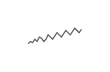
\begin{tikzpicture}[x=0.08em, y=0.08em, line width=0.4pt]
                \draw[FooterGray] (0,3) -- (1,4) -- (2,3.5) -- (3,5) -- (4,4) -- (5,6) -- (6,5.5) -- (7,4) -- (8,5) -- (9,7) -- (10,6) -- (11,5) -- (12,6.5) -- (13,8) -- (14,7) -- (15,6) -- (16,7.5) -- (17,9) -- (18,8) -- (19,7) -- (20,8.5) -- (21,10) -- (22,9) -- (23,8) -- (24,9.5);
            \end{tikzpicture}%
        }%
        \hskip0.5cm%
    }%
    \vskip6pt%
}

%=============================================================================
% PACKAGES
%=============================================================================
\usepackage[utf8]{inputenc}
\DeclareUnicodeCharacter{03B1}{\ensuremath{\alpha}}
\usepackage[T1]{fontenc}
\usepackage{amsmath, amssymb, amsthm}
\usepackage{mathtools}
\usepackage{bm}
\usepackage{tikz}
\usetikzlibrary{arrows.meta, positioning, shapes, calc, decorations.pathreplacing, shadings}
\usepackage{booktabs}
\usepackage{multirow}
\usepackage{array}
\usepackage{graphicx}
\usepackage{animate}
\usepackage{hyperref}
\usepackage{colortbl}
\usepackage{listings}
\lstset{language=Python, basicstyle=\ttfamily\scriptsize, keywordstyle=\color{MainBlue}\bfseries,
  commentstyle=\color{Forest}, stringstyle=\color{Crimson}, breaklines=true,
  frame=none, backgroundcolor=\color{VeryLightGray}, xleftmargin=2mm}
\hypersetup{colorlinks=true, linkcolor=MainBlue, urlcolor=MainBlue}
\graphicspath{{../../logos/}{../../charts/}{../../photos/}}
\usepackage{xcolor}
\hfuzz=2pt  % Suppress tiny overfull warnings (<2pt)
\vfuzz=2pt  % Suppress tiny vertical overfull warnings (<2pt)
% \mathrm in the sans-serif family of the slides (beamer resets \mathrm to the serif family at \begin{document};
% this hook runs after beamer's, so WN, Var, RMSE, ... in formulas match the surrounding text)
% Bold vectors and matrices in the same sans-serif family: \mathbf{A} in sans bold (beamer's own \mathbf came out in
% medium weight), and the bold upright Greek capitals of \boldsymbol / \bm (\bSigma, \bPhi, \boldsymbol{\Theta}) in
% cmss bold: bm.sty fixes its "boldoperators" font when it is loaded (serif cmbx), before beamer switches the
% operators to cmss, so it is reset here.
\AtBeginDocument{%
  \SetMathAlphabet{\mathrm}{normal}{\encodingdefault}{\sfdefault}{\mddefault}{n}%
  \SetMathAlphabet{\mathrm}{bold}{\encodingdefault}{\sfdefault}{bx}{n}%
  \SetMathAlphabet{\mathbf}{normal}{\encodingdefault}{\sfdefault}{bx}{n}%
  \SetMathAlphabet{\mathbf}{bold}{\encodingdefault}{\sfdefault}{bx}{n}%
  \SetSymbolFont{boldoperators}{normal}{OT1}{cmss}{bx}{n}%
  \SetSymbolFont{boldoperators}{bold}{OT1}{cmss}{bx}{n}}

%=============================================================================
% QUANTLET COMMANDS
%   \quantlet{<displayed name>}{<url>}       (generic, compatible with the older TSA decks)
%   \tsaquantlet{Ch_05}{TSA_ch5_garch}       -> https://github.com/danpele/Time-Series-Analysis/tree/main/Quantlets/Ch_05/TSA_ch5_garch
%   \qlurl{<folder>} is defined per chapter by the generator (Quantlets/Ch_NN/<folder>)
%=============================================================================
\newcommand{\tsarepo}{https://github.com/danpele/Time-Series-Analysis}
\newcommand{\tsaqlbase}{https://github.com/danpele/Time-Series-Analysis/tree/main/Quantlets}
\newcommand{\quantlet}[2]{%
    \hfill\href{#2}{%
        \raisebox{-0.15em}{
\includegraphics[height=0.7em]{ql_logo.png}}%
        \textcolor{MainBlue}{\tiny\ #1}%
    }%
}
\newcommand{\tsaquantlet}[2]{\quantlet{\detokenize{#2}}{\tsaqlbase/#1/#2}}

%=============================================================================
% NOTEBOOKS (Google Colab)
%   \colaburl{notebooks/EN/chapter5_seminar_notebook.ipynb} -> the Colab link of a file in the TSA repo
%   \nb: the chapter notebook (each seminar deck redefines it with \renewcommand)
%=============================================================================
\newcommand{\colaburl}[1]{https://colab.research.google.com/github/danpele/Time-Series-Analysis/blob/main/#1}
\newcommand{\nb}{https://colab.research.google.com/github/danpele/Time-Series-Analysis/tree/main/notebooks/EN}
\newcommand{\nbname}{notebooks/EN}

%=============================================================================
% SLIDE HELPERS (used by the generators; the same as in MFM)
%=============================================================================
% local font size for list bodies (the preamble forces \normalsize)
\newcommand{\itemsize}[1]{\setbeamertemplate{itemize/enumerate body begin}{#1}\setbeamertemplate{itemize/enumerate subbody begin}{#1}}
\newcommand{\intitle}[1]{{\hypersetup{urlcolor=white}#1}}   % white links inside coloured title bars
\newcommand{\imgcap}[1]{{\scriptsize #1}\\[0.5mm]}          % caption under a photo
\newcommand{\imgcredit}[2]{{\tiny\color{FooterGray}\href{#1}{#2}}}   % image credit: source URL, author/licence
\newcommand{\aiprompt}[1]{{\ttfamily\color{MainBlue}#1}}     % a prompt to an AI assistant

%=============================================================================
% SEMINARS: student version by default; the instructor wrapper *_solutions.tex sets \solutionstrue
%=============================================================================
\makeatletter\@ifundefined{ifsolutions}{\expandafter\newif\csname ifsolutions\endcsname}{}\makeatother
\newcommand{\solonly}[1]{\ifsolutions #1\fi}
\newcommand{\propsub}{\ifsolutions\else\framesubtitle{\ifdefined\tsalang Rezolvarea se discută la seminar\else Solution discussed in class\fi}\fi}

%=============================================================================
% APPENDIX AND CHAPTER LINKS (latex/appendix_links.py writes the calls; it also re-declares these
% macros before \begin{document}, so the decks compile with or without this preamble block)
%=============================================================================
\providecommand{\tsaapplink}[3]{\hypertarget{#2}{}\hyperlink{#1}{\beamergotobutton{#3}}}
\providecommand{\tsaappback}[2]{\begin{tikzpicture}[remember picture,overlay]\node[anchor=south east] at ([xshift=-3mm,yshift=7mm]current page.south east){\hyperlink{#1}{\beamerreturnbutton{#2}}};\end{tikzpicture}}
\providecommand{\tsachlink}[2]{\href{#1}{#2}}
\providecommand{\tsachlinkt}[2]{\href{#1}{\usebeamercolor[fg]{frametitle}#2}}

%=============================================================================
% QUANTINAR COMMAND: link către un curs Quantinar (subiecte avansate)
%=============================================================================
\newcommand{\quantinar}[2]{%
    \href{#2}{%
        \raisebox{-0.15em}{
\includegraphics[height=0.8em]{qr_logo.png}}%
        \textcolor{MainBlue}{\scriptsize\ #1}%
    }%
}

%=============================================================================
% CUSTOM TITLE PAGE
%=============================================================================
\defbeamertemplate*{title page}{hybrid}[1][]
{
    \vspace{0.2cm}
    % Logos row - top header (with clickable links)
    \begin{center}
        \href{https://www.ase.ro}{
\includegraphics[height=1.0cm]{ase_logo.png}}\hspace{0.3cm}%
        \href{https://theida.net}{
\includegraphics[height=1.0cm]{ida_logo.png}}\hspace{0.3cm}%
        \href{https://blockchain-research-center.com}{
\includegraphics[height=1.0cm]{brc_logo.png}}\hspace{0.3cm}%
        \href{https://www.ai4efin.ase.ro}{
\includegraphics[height=1.0cm]{ai4efin_logo.png}}\hspace{0.3cm}%
        \href{https://ipe.ro/new}{
\includegraphics[height=1.0cm]{acad_logo.png}}\hspace{0.3cm}%
        \href{https://www.digital-finance-msca.com}{
\includegraphics[height=1.0cm]{msca_logo.png}}%
    \end{center}

    \vspace{0.6cm}

    % Main title with Q logos on sides (with clickable links)
    \begin{center}
        \begin{minipage}{0.1\textwidth}
            \centering
            \href{https://quantlet.com}{
\includegraphics[height=1.1cm]{ql_logo.png}}
        \end{minipage}%
        \begin{minipage}{0.78\textwidth}
            \centering
            {\LARGE\bfseries\usebeamercolor[fg]{title}\inserttitle}

            \vspace{0.3cm}

            {\usebeamerfont{subtitle}\usebeamercolor[fg]{title}\insertsubtitle}
        \end{minipage}%
        \begin{minipage}{0.1\textwidth}
            \centering
            \href{https://quantinar.com}{
\includegraphics[height=1.1cm]{qr_logo.png}}
        \end{minipage}
    \end{center}

    \vspace{0.6cm}

    % Authors (left aligned)
    \hspace{0.5cm}{\usebeamerfont{author}\insertauthor}

    \vspace{0.3cm}

    % Institute/Affiliations (left aligned)
    \hspace{0.5cm}\begin{minipage}[t]{0.9\textwidth}
        \raggedright\small\insertinstitute
    \end{minipage}
}

%=============================================================================
% THEOREM ENVIRONMENTS
%=============================================================================
\theoremstyle{definition}
\setbeamertemplate{theorems}[numbered]
\ifdefined\tsalang
\newtheorem{defn}{Definiție}
\newtheorem{thm}{Teoremă}
\newtheorem{prop}{Propoziție}
\newtheorem{rmk}{Observație}
\else
\newtheorem{defn}{Definition}
\newtheorem{thm}{Theorem}
\newtheorem{prop}{Proposition}
\newtheorem{rmk}{Remark}
\fi

%=============================================================================
% CENTRED MINIPAGE (no extra vertical space)
%=============================================================================
\newenvironment{cminipage}[1]{%
    \par\noindent\hfill\begin{minipage}{#1}\ignorespaces
}{%
    \end{minipage}\hfill\null\par
}

%=============================================================================
% CUSTOM COMMANDS
%=============================================================================
\newcommand{\E}{\mathbb{E}}
\newcommand{\Var}{\text{Var}}
\newcommand{\Cov}{\text{Cov}}
\newcommand{\Corr}{\text{Corr}}
\newcommand{\R}{\mathbb{R}}
\newcommand{\N}{\mathbb{N}}
\newcommand{\Z}{\mathbb{Z}}
\newcommand{\B}{\mathbf{B}}
\newcommand{\imark}{\textcolor{MainBlue}{\textbullet}}
\newcommand{\RMSE}{\text{RMSE}}
\newcommand{\MAE}{\text{MAE}}
\newcommand{\MAPE}{\text{MAPE}}

% Boldface vector/matrix commands (VAR, VECM, state space; also used by the older TSA decks)
\newcommand{\bY}{\mathbf{Y}}
\newcommand{\bX}{\mathbf{X}}
\newcommand{\bA}{\mathbf{A}}
\newcommand{\bB}{\mathbf{B}}
\newcommand{\bepsilon}{\boldsymbol{\varepsilon}}
\newcommand{\bSigma}{\boldsymbol{\Sigma}}
\newcommand{\bPhi}{\boldsymbol{\Phi}}
\newcommand{\bGamma}{\boldsymbol{\Gamma}}
\newcommand{\bPi}{\boldsymbol{\Pi}}
\newcommand{\bc}{\mathbf{c}}
\newcommand{\balpha}{\boldsymbol{\alpha}}
\newcommand{\bbeta}{\boldsymbol{\beta}}
\newcommand{\bvarepsilon}{\boldsymbol{\varepsilon}}

% Legacy seminar marks (older TSA seminar decks)
\newcommand{\correct}{\textcolor{Forest}{\checkmark}}
\newcommand{\incorrect}{\textcolor{Crimson}{\texttimes}}
 se definește
%   \newcommand{\coursename}{Time Series Analysis}      (EN)
%   \newcommand{\coursename}{Serii de timp}       (RO)  și  \def\tsalang{ro}
% Fișierele .tex se află în EN/Courses, EN/Seminars, RO/Cursuri, RO/Seminarii (două niveluri sub rădăcină).
% Deck-urile sînt generate de latex/build_chapterN.py / build_seminarN.py (vezi latex/tsa_build.py).

\documentclass[9pt, aspectratio=169, t]{beamer}
\providecommand{\coursename}{Time Series Analysis}

% Ensure content fits on slides
\setbeamersize{text margin left=8mm, text margin right=8mm}
% Smaller institute font (title page)
\setbeamerfont{institute}{size=\footnotesize}

%=============================================================================
% THEME AND STYLE CONFIGURATION
%=============================================================================
\usetheme{default}
% Using default theme for clean header/footer control

% Color Palette (matching Redispatch PDF)
\definecolor{MainBlue}{RGB}{26, 58, 110}
\definecolor{AccentBlue}{RGB}{26, 58, 110}
\definecolor{IDAred}{RGB}{205, 0, 0}
\definecolor{DarkGray}{RGB}{51, 51, 51}
\definecolor{MediumGray}{RGB}{128, 128, 128}
\definecolor{LightGray}{RGB}{248, 248, 248}
\definecolor{VeryLightGray}{RGB}{235, 235, 235}
\definecolor{KeynoteGray}{RGB}{218, 218, 218}
\definecolor{SectionGray}{RGB}{120, 120, 120}
\definecolor{FooterGray}{RGB}{100, 100, 100}
\definecolor{Crimson}{RGB}{220, 53, 69}
\definecolor{Forest}{RGB}{46, 125, 50}
\definecolor{Amber}{RGB}{181, 133, 63}
\definecolor{Orange}{RGB}{230, 126, 34}
\definecolor{Purple}{RGB}{142, 68, 173}

% Gradient background (exact Keynote 315° gradient: white to RGB 218,218,218)
\setbeamertemplate{background}{%
    \begin{tikzpicture}[remember picture, overlay]
        \shade[shading=axis, shading angle=315,
        top color=white, bottom color=KeynoteGray]
        (current page.south west) rectangle (current page.north east);
    \end{tikzpicture}%
}
% Fallback solid color for compatibility
\setbeamercolor{background canvas}{bg=}

\setbeamercolor{palette primary}{bg=MainBlue, fg=white}
\setbeamercolor{palette secondary}{bg=MainBlue!85, fg=white}
\setbeamercolor{palette tertiary}{bg=MainBlue!70, fg=white}
\setbeamercolor{structure}{fg=MainBlue}
\setbeamercolor{title}{fg=IDAred}
\setbeamercolor{frametitle}{fg=IDAred, bg=}
\setbeamercolor{block title}{bg=MainBlue, fg=white}
\setbeamercolor{block body}{bg=VeryLightGray, fg=DarkGray}
\setbeamercolor{block title alerted}{bg=Crimson, fg=white}
\setbeamercolor{block body alerted}{bg=Crimson!8, fg=DarkGray}
\setbeamercolor{block title example}{bg=Forest, fg=white}
\setbeamercolor{block body example}{bg=Forest!8, fg=DarkGray}
\setbeamercolor{item}{fg=MainBlue}

% Footer colors (override Madrid theme blue)
\setbeamercolor{author in head/foot}{fg=FooterGray, bg=}
\setbeamercolor{title in head/foot}{fg=FooterGray, bg=}
\setbeamercolor{date in head/foot}{fg=FooterGray, bg=}
\setbeamercolor{section in head/foot}{fg=FooterGray, bg=}
\setbeamercolor{subsection in head/foot}{fg=FooterGray, bg=}

% Bullet styles (apply everywhere including blocks)
\setbeamertemplate{itemize item}{\color{MainBlue}$\boxdot$}
\setbeamertemplate{itemize subitem}{\color{MainBlue}$\blacktriangleright$}
\setbeamertemplate{itemize subsubitem}{\color{MainBlue}\tiny$\bullet$}
\setbeamertemplate{itemize/enumerate body begin}{\normalsize}
\setbeamertemplate{itemize/enumerate subbody begin}{\normalsize}

% Item spacing - compact style
\setlength{\leftmargini}{10pt}       % Level 1: minimal indent
\setlength{\leftmarginii}{10pt}      % Level 2: minimal additional indent
% Compact list spacing (zero extra space before/after lists in blocks)
\makeatletter
\def\@listi{\leftmargin\leftmargini \topsep 0pt \parsep 0pt \itemsep 0pt}
\def\@listii{\leftmargin\leftmarginii \topsep 0pt \parsep 0pt \itemsep 0pt}
\makeatother

\setbeamertemplate{navigation symbols}{}

%=============================================================================
% CUSTOM HEADLINE
%=============================================================================
\setbeamertemplate{headline}{%
    \vskip10pt%
    \hbox to \paperwidth{%
        \hskip0.5cm%
        {\small\color{FooterGray}\renewcommand{\hyperlink}[2]{##2}\insertsectionhead}%
        \hfill%
        \textcolor{FooterGray}{\small\insertframenumber}%
        \hskip0.5cm%
    }%
    \vskip4pt%
    {\color{FooterGray}\hrule height 0.4pt}%
}

%=============================================================================
% CUSTOM FOOTER
%=============================================================================
\usepackage{fontawesome5}

\setbeamertemplate{footline}{%
    {\color{FooterGray}\hrule height 0.4pt}%
    \vskip4pt%
    \hbox to \paperwidth{%
        \hskip0.5cm%
        \textcolor{FooterGray}{\small\coursename}%
        \hfill%
        \raisebox{-0.1em}{%
            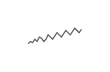
\begin{tikzpicture}[x=0.08em, y=0.08em, line width=0.4pt]
                \draw[FooterGray] (0,3) -- (1,4) -- (2,3.5) -- (3,5) -- (4,4) -- (5,6) -- (6,5.5) -- (7,4) -- (8,5) -- (9,7) -- (10,6) -- (11,5) -- (12,6.5) -- (13,8) -- (14,7) -- (15,6) -- (16,7.5) -- (17,9) -- (18,8) -- (19,7) -- (20,8.5) -- (21,10) -- (22,9) -- (23,8) -- (24,9.5);
            \end{tikzpicture}%
        }%
        \hskip0.5cm%
    }%
    \vskip6pt%
}

%=============================================================================
% PACKAGES
%=============================================================================
\usepackage[utf8]{inputenc}
\DeclareUnicodeCharacter{03B1}{\ensuremath{\alpha}}
\usepackage[T1]{fontenc}
\usepackage{amsmath, amssymb, amsthm}
\usepackage{mathtools}
\usepackage{bm}
\usepackage{tikz}
\usetikzlibrary{arrows.meta, positioning, shapes, calc, decorations.pathreplacing, shadings}
\usepackage{booktabs}
\usepackage{multirow}
\usepackage{array}
\usepackage{graphicx}
\usepackage{animate}
\usepackage{hyperref}
\usepackage{colortbl}
\usepackage{listings}
\lstset{language=Python, basicstyle=\ttfamily\scriptsize, keywordstyle=\color{MainBlue}\bfseries,
  commentstyle=\color{Forest}, stringstyle=\color{Crimson}, breaklines=true,
  frame=none, backgroundcolor=\color{VeryLightGray}, xleftmargin=2mm}
\hypersetup{colorlinks=true, linkcolor=MainBlue, urlcolor=MainBlue}
\graphicspath{{../../logos/}{../../charts/}{../../photos/}}
\usepackage{xcolor}
\hfuzz=2pt  % Suppress tiny overfull warnings (<2pt)
\vfuzz=2pt  % Suppress tiny vertical overfull warnings (<2pt)
% \mathrm in the sans-serif family of the slides (beamer resets \mathrm to the serif family at \begin{document};
% this hook runs after beamer's, so WN, Var, RMSE, ... in formulas match the surrounding text)
% Bold vectors and matrices in the same sans-serif family: \mathbf{A} in sans bold (beamer's own \mathbf came out in
% medium weight), and the bold upright Greek capitals of \boldsymbol / \bm (\bSigma, \bPhi, \boldsymbol{\Theta}) in
% cmss bold: bm.sty fixes its "boldoperators" font when it is loaded (serif cmbx), before beamer switches the
% operators to cmss, so it is reset here.
\AtBeginDocument{%
  \SetMathAlphabet{\mathrm}{normal}{\encodingdefault}{\sfdefault}{\mddefault}{n}%
  \SetMathAlphabet{\mathrm}{bold}{\encodingdefault}{\sfdefault}{bx}{n}%
  \SetMathAlphabet{\mathbf}{normal}{\encodingdefault}{\sfdefault}{bx}{n}%
  \SetMathAlphabet{\mathbf}{bold}{\encodingdefault}{\sfdefault}{bx}{n}%
  \SetSymbolFont{boldoperators}{normal}{OT1}{cmss}{bx}{n}%
  \SetSymbolFont{boldoperators}{bold}{OT1}{cmss}{bx}{n}}

%=============================================================================
% QUANTLET COMMANDS
%   \quantlet{<displayed name>}{<url>}       (generic, compatible with the older TSA decks)
%   \tsaquantlet{Ch_05}{TSA_ch5_garch}       -> https://github.com/danpele/Time-Series-Analysis/tree/main/Quantlets/Ch_05/TSA_ch5_garch
%   \qlurl{<folder>} is defined per chapter by the generator (Quantlets/Ch_NN/<folder>)
%=============================================================================
\newcommand{\tsarepo}{https://github.com/danpele/Time-Series-Analysis}
\newcommand{\tsaqlbase}{https://github.com/danpele/Time-Series-Analysis/tree/main/Quantlets}
\newcommand{\quantlet}[2]{%
    \hfill\href{#2}{%
        \raisebox{-0.15em}{
\includegraphics[height=0.7em]{ql_logo.png}}%
        \textcolor{MainBlue}{\tiny\ #1}%
    }%
}
\newcommand{\tsaquantlet}[2]{\quantlet{\detokenize{#2}}{\tsaqlbase/#1/#2}}

%=============================================================================
% NOTEBOOKS (Google Colab)
%   \colaburl{notebooks/EN/chapter5_seminar_notebook.ipynb} -> the Colab link of a file in the TSA repo
%   \nb: the chapter notebook (each seminar deck redefines it with \renewcommand)
%=============================================================================
\newcommand{\colaburl}[1]{https://colab.research.google.com/github/danpele/Time-Series-Analysis/blob/main/#1}
\newcommand{\nb}{https://colab.research.google.com/github/danpele/Time-Series-Analysis/tree/main/notebooks/EN}
\newcommand{\nbname}{notebooks/EN}

%=============================================================================
% SLIDE HELPERS (used by the generators; the same as in MFM)
%=============================================================================
% local font size for list bodies (the preamble forces \normalsize)
\newcommand{\itemsize}[1]{\setbeamertemplate{itemize/enumerate body begin}{#1}\setbeamertemplate{itemize/enumerate subbody begin}{#1}}
\newcommand{\intitle}[1]{{\hypersetup{urlcolor=white}#1}}   % white links inside coloured title bars
\newcommand{\imgcap}[1]{{\scriptsize #1}\\[0.5mm]}          % caption under a photo
\newcommand{\imgcredit}[2]{{\tiny\color{FooterGray}\href{#1}{#2}}}   % image credit: source URL, author/licence
\newcommand{\aiprompt}[1]{{\ttfamily\color{MainBlue}#1}}     % a prompt to an AI assistant

%=============================================================================
% SEMINARS: student version by default; the instructor wrapper *_solutions.tex sets \solutionstrue
%=============================================================================
\makeatletter\@ifundefined{ifsolutions}{\expandafter\newif\csname ifsolutions\endcsname}{}\makeatother
\newcommand{\solonly}[1]{\ifsolutions #1\fi}
\newcommand{\propsub}{\ifsolutions\else\framesubtitle{\ifdefined\tsalang Rezolvarea se discută la seminar\else Solution discussed in class\fi}\fi}

%=============================================================================
% APPENDIX AND CHAPTER LINKS (latex/appendix_links.py writes the calls; it also re-declares these
% macros before \begin{document}, so the decks compile with or without this preamble block)
%=============================================================================
\providecommand{\tsaapplink}[3]{\hypertarget{#2}{}\hyperlink{#1}{\beamergotobutton{#3}}}
\providecommand{\tsaappback}[2]{\begin{tikzpicture}[remember picture,overlay]\node[anchor=south east] at ([xshift=-3mm,yshift=7mm]current page.south east){\hyperlink{#1}{\beamerreturnbutton{#2}}};\end{tikzpicture}}
\providecommand{\tsachlink}[2]{\href{#1}{#2}}
\providecommand{\tsachlinkt}[2]{\href{#1}{\usebeamercolor[fg]{frametitle}#2}}

%=============================================================================
% QUANTINAR COMMAND: link către un curs Quantinar (subiecte avansate)
%=============================================================================
\newcommand{\quantinar}[2]{%
    \href{#2}{%
        \raisebox{-0.15em}{
\includegraphics[height=0.8em]{qr_logo.png}}%
        \textcolor{MainBlue}{\scriptsize\ #1}%
    }%
}

%=============================================================================
% CUSTOM TITLE PAGE
%=============================================================================
\defbeamertemplate*{title page}{hybrid}[1][]
{
    \vspace{0.2cm}
    % Logos row - top header (with clickable links)
    \begin{center}
        \href{https://www.ase.ro}{
\includegraphics[height=1.0cm]{ase_logo.png}}\hspace{0.3cm}%
        \href{https://theida.net}{
\includegraphics[height=1.0cm]{ida_logo.png}}\hspace{0.3cm}%
        \href{https://blockchain-research-center.com}{
\includegraphics[height=1.0cm]{brc_logo.png}}\hspace{0.3cm}%
        \href{https://www.ai4efin.ase.ro}{
\includegraphics[height=1.0cm]{ai4efin_logo.png}}\hspace{0.3cm}%
        \href{https://ipe.ro/new}{
\includegraphics[height=1.0cm]{acad_logo.png}}\hspace{0.3cm}%
        \href{https://www.digital-finance-msca.com}{
\includegraphics[height=1.0cm]{msca_logo.png}}%
    \end{center}

    \vspace{0.6cm}

    % Main title with Q logos on sides (with clickable links)
    \begin{center}
        \begin{minipage}{0.1\textwidth}
            \centering
            \href{https://quantlet.com}{
\includegraphics[height=1.1cm]{ql_logo.png}}
        \end{minipage}%
        \begin{minipage}{0.78\textwidth}
            \centering
            {\LARGE\bfseries\usebeamercolor[fg]{title}\inserttitle}

            \vspace{0.3cm}

            {\usebeamerfont{subtitle}\usebeamercolor[fg]{title}\insertsubtitle}
        \end{minipage}%
        \begin{minipage}{0.1\textwidth}
            \centering
            \href{https://quantinar.com}{
\includegraphics[height=1.1cm]{qr_logo.png}}
        \end{minipage}
    \end{center}

    \vspace{0.6cm}

    % Authors (left aligned)
    \hspace{0.5cm}{\usebeamerfont{author}\insertauthor}

    \vspace{0.3cm}

    % Institute/Affiliations (left aligned)
    \hspace{0.5cm}\begin{minipage}[t]{0.9\textwidth}
        \raggedright\small\insertinstitute
    \end{minipage}
}

%=============================================================================
% THEOREM ENVIRONMENTS
%=============================================================================
\theoremstyle{definition}
\setbeamertemplate{theorems}[numbered]
\ifdefined\tsalang
\newtheorem{defn}{Definiție}
\newtheorem{thm}{Teoremă}
\newtheorem{prop}{Propoziție}
\newtheorem{rmk}{Observație}
\else
\newtheorem{defn}{Definition}
\newtheorem{thm}{Theorem}
\newtheorem{prop}{Proposition}
\newtheorem{rmk}{Remark}
\fi

%=============================================================================
% CENTRED MINIPAGE (no extra vertical space)
%=============================================================================
\newenvironment{cminipage}[1]{%
    \par\noindent\hfill\begin{minipage}{#1}\ignorespaces
}{%
    \end{minipage}\hfill\null\par
}

%=============================================================================
% CUSTOM COMMANDS
%=============================================================================
\newcommand{\E}{\mathbb{E}}
\newcommand{\Var}{\text{Var}}
\newcommand{\Cov}{\text{Cov}}
\newcommand{\Corr}{\text{Corr}}
\newcommand{\R}{\mathbb{R}}
\newcommand{\N}{\mathbb{N}}
\newcommand{\Z}{\mathbb{Z}}
\newcommand{\B}{\mathbf{B}}
\newcommand{\imark}{\textcolor{MainBlue}{\textbullet}}
\newcommand{\RMSE}{\text{RMSE}}
\newcommand{\MAE}{\text{MAE}}
\newcommand{\MAPE}{\text{MAPE}}

% Boldface vector/matrix commands (VAR, VECM, state space; also used by the older TSA decks)
\newcommand{\bY}{\mathbf{Y}}
\newcommand{\bX}{\mathbf{X}}
\newcommand{\bA}{\mathbf{A}}
\newcommand{\bB}{\mathbf{B}}
\newcommand{\bepsilon}{\boldsymbol{\varepsilon}}
\newcommand{\bSigma}{\boldsymbol{\Sigma}}
\newcommand{\bPhi}{\boldsymbol{\Phi}}
\newcommand{\bGamma}{\boldsymbol{\Gamma}}
\newcommand{\bPi}{\boldsymbol{\Pi}}
\newcommand{\bc}{\mathbf{c}}
\newcommand{\balpha}{\boldsymbol{\alpha}}
\newcommand{\bbeta}{\boldsymbol{\beta}}
\newcommand{\bvarepsilon}{\boldsymbol{\varepsilon}}

% Legacy seminar marks (older TSA seminar decks)
\newcommand{\correct}{\textcolor{Forest}{\checkmark}}
\newcommand{\incorrect}{\textcolor{Crimson}{\texttimes}}
 se definește
%   \newcommand{\coursename}{Time Series Analysis}      (EN)
%   \newcommand{\coursename}{Serii de timp}       (RO)  și  \def\tsalang{ro}
% Fișierele .tex se află în EN/Courses, EN/Seminars, RO/Cursuri, RO/Seminarii (două niveluri sub rădăcină).
% Deck-urile sînt generate de latex/build_chapterN.py / build_seminarN.py (vezi latex/tsa_build.py).

\documentclass[9pt, aspectratio=169, t]{beamer}
\providecommand{\coursename}{Time Series Analysis}

% Ensure content fits on slides
\setbeamersize{text margin left=8mm, text margin right=8mm}
% Smaller institute font (title page)
\setbeamerfont{institute}{size=\footnotesize}

%=============================================================================
% THEME AND STYLE CONFIGURATION
%=============================================================================
\usetheme{default}
% Using default theme for clean header/footer control

% Color Palette (matching Redispatch PDF)
\definecolor{MainBlue}{RGB}{26, 58, 110}
\definecolor{AccentBlue}{RGB}{26, 58, 110}
\definecolor{IDAred}{RGB}{205, 0, 0}
\definecolor{DarkGray}{RGB}{51, 51, 51}
\definecolor{MediumGray}{RGB}{128, 128, 128}
\definecolor{LightGray}{RGB}{248, 248, 248}
\definecolor{VeryLightGray}{RGB}{235, 235, 235}
\definecolor{KeynoteGray}{RGB}{218, 218, 218}
\definecolor{SectionGray}{RGB}{120, 120, 120}
\definecolor{FooterGray}{RGB}{100, 100, 100}
\definecolor{Crimson}{RGB}{220, 53, 69}
\definecolor{Forest}{RGB}{46, 125, 50}
\definecolor{Amber}{RGB}{181, 133, 63}
\definecolor{Orange}{RGB}{230, 126, 34}
\definecolor{Purple}{RGB}{142, 68, 173}

% Gradient background (exact Keynote 315° gradient: white to RGB 218,218,218)
\setbeamertemplate{background}{%
    \begin{tikzpicture}[remember picture, overlay]
        \shade[shading=axis, shading angle=315,
        top color=white, bottom color=KeynoteGray]
        (current page.south west) rectangle (current page.north east);
    \end{tikzpicture}%
}
% Fallback solid color for compatibility
\setbeamercolor{background canvas}{bg=}

\setbeamercolor{palette primary}{bg=MainBlue, fg=white}
\setbeamercolor{palette secondary}{bg=MainBlue!85, fg=white}
\setbeamercolor{palette tertiary}{bg=MainBlue!70, fg=white}
\setbeamercolor{structure}{fg=MainBlue}
\setbeamercolor{title}{fg=IDAred}
\setbeamercolor{frametitle}{fg=IDAred, bg=}
\setbeamercolor{block title}{bg=MainBlue, fg=white}
\setbeamercolor{block body}{bg=VeryLightGray, fg=DarkGray}
\setbeamercolor{block title alerted}{bg=Crimson, fg=white}
\setbeamercolor{block body alerted}{bg=Crimson!8, fg=DarkGray}
\setbeamercolor{block title example}{bg=Forest, fg=white}
\setbeamercolor{block body example}{bg=Forest!8, fg=DarkGray}
\setbeamercolor{item}{fg=MainBlue}

% Footer colors (override Madrid theme blue)
\setbeamercolor{author in head/foot}{fg=FooterGray, bg=}
\setbeamercolor{title in head/foot}{fg=FooterGray, bg=}
\setbeamercolor{date in head/foot}{fg=FooterGray, bg=}
\setbeamercolor{section in head/foot}{fg=FooterGray, bg=}
\setbeamercolor{subsection in head/foot}{fg=FooterGray, bg=}

% Bullet styles (apply everywhere including blocks)
\setbeamertemplate{itemize item}{\color{MainBlue}$\boxdot$}
\setbeamertemplate{itemize subitem}{\color{MainBlue}$\blacktriangleright$}
\setbeamertemplate{itemize subsubitem}{\color{MainBlue}\tiny$\bullet$}
\setbeamertemplate{itemize/enumerate body begin}{\normalsize}
\setbeamertemplate{itemize/enumerate subbody begin}{\normalsize}

% Item spacing - compact style
\setlength{\leftmargini}{10pt}       % Level 1: minimal indent
\setlength{\leftmarginii}{10pt}      % Level 2: minimal additional indent
% Compact list spacing (zero extra space before/after lists in blocks)
\makeatletter
\def\@listi{\leftmargin\leftmargini \topsep 0pt \parsep 0pt \itemsep 0pt}
\def\@listii{\leftmargin\leftmarginii \topsep 0pt \parsep 0pt \itemsep 0pt}
\makeatother

\setbeamertemplate{navigation symbols}{}

%=============================================================================
% CUSTOM HEADLINE
%=============================================================================
\setbeamertemplate{headline}{%
    \vskip10pt%
    \hbox to \paperwidth{%
        \hskip0.5cm%
        {\small\color{FooterGray}\renewcommand{\hyperlink}[2]{##2}\insertsectionhead}%
        \hfill%
        \textcolor{FooterGray}{\small\insertframenumber}%
        \hskip0.5cm%
    }%
    \vskip4pt%
    {\color{FooterGray}\hrule height 0.4pt}%
}

%=============================================================================
% CUSTOM FOOTER
%=============================================================================
\usepackage{fontawesome5}

\setbeamertemplate{footline}{%
    {\color{FooterGray}\hrule height 0.4pt}%
    \vskip4pt%
    \hbox to \paperwidth{%
        \hskip0.5cm%
        \textcolor{FooterGray}{\small\coursename}%
        \hfill%
        \raisebox{-0.1em}{%
            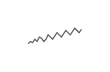
\begin{tikzpicture}[x=0.08em, y=0.08em, line width=0.4pt]
                \draw[FooterGray] (0,3) -- (1,4) -- (2,3.5) -- (3,5) -- (4,4) -- (5,6) -- (6,5.5) -- (7,4) -- (8,5) -- (9,7) -- (10,6) -- (11,5) -- (12,6.5) -- (13,8) -- (14,7) -- (15,6) -- (16,7.5) -- (17,9) -- (18,8) -- (19,7) -- (20,8.5) -- (21,10) -- (22,9) -- (23,8) -- (24,9.5);
            \end{tikzpicture}%
        }%
        \hskip0.5cm%
    }%
    \vskip6pt%
}

%=============================================================================
% PACKAGES
%=============================================================================
\usepackage[utf8]{inputenc}
\DeclareUnicodeCharacter{03B1}{\ensuremath{\alpha}}
\usepackage[T1]{fontenc}
\usepackage{amsmath, amssymb, amsthm}
\usepackage{mathtools}
\usepackage{bm}
\usepackage{tikz}
\usetikzlibrary{arrows.meta, positioning, shapes, calc, decorations.pathreplacing, shadings}
\usepackage{booktabs}
\usepackage{multirow}
\usepackage{array}
\usepackage{graphicx}
\usepackage{animate}
\usepackage{hyperref}
\usepackage{colortbl}
\usepackage{listings}
\lstset{language=Python, basicstyle=\ttfamily\scriptsize, keywordstyle=\color{MainBlue}\bfseries,
  commentstyle=\color{Forest}, stringstyle=\color{Crimson}, breaklines=true,
  frame=none, backgroundcolor=\color{VeryLightGray}, xleftmargin=2mm}
\hypersetup{colorlinks=true, linkcolor=MainBlue, urlcolor=MainBlue}
\graphicspath{{../../logos/}{../../charts/}{../../photos/}}
\usepackage{xcolor}
\hfuzz=2pt  % Suppress tiny overfull warnings (<2pt)
\vfuzz=2pt  % Suppress tiny vertical overfull warnings (<2pt)
% \mathrm in the sans-serif family of the slides (beamer resets \mathrm to the serif family at \begin{document};
% this hook runs after beamer's, so WN, Var, RMSE, ... in formulas match the surrounding text)
% Bold vectors and matrices in the same sans-serif family: \mathbf{A} in sans bold (beamer's own \mathbf came out in
% medium weight), and the bold upright Greek capitals of \boldsymbol / \bm (\bSigma, \bPhi, \boldsymbol{\Theta}) in
% cmss bold: bm.sty fixes its "boldoperators" font when it is loaded (serif cmbx), before beamer switches the
% operators to cmss, so it is reset here.
\AtBeginDocument{%
  \SetMathAlphabet{\mathrm}{normal}{\encodingdefault}{\sfdefault}{\mddefault}{n}%
  \SetMathAlphabet{\mathrm}{bold}{\encodingdefault}{\sfdefault}{bx}{n}%
  \SetMathAlphabet{\mathbf}{normal}{\encodingdefault}{\sfdefault}{bx}{n}%
  \SetMathAlphabet{\mathbf}{bold}{\encodingdefault}{\sfdefault}{bx}{n}%
  \SetSymbolFont{boldoperators}{normal}{OT1}{cmss}{bx}{n}%
  \SetSymbolFont{boldoperators}{bold}{OT1}{cmss}{bx}{n}}

%=============================================================================
% QUANTLET COMMANDS
%   \quantlet{<displayed name>}{<url>}       (generic, compatible with the older TSA decks)
%   \tsaquantlet{Ch_05}{TSA_ch5_garch}       -> https://github.com/danpele/Time-Series-Analysis/tree/main/Quantlets/Ch_05/TSA_ch5_garch
%   \qlurl{<folder>} is defined per chapter by the generator (Quantlets/Ch_NN/<folder>)
%=============================================================================
\newcommand{\tsarepo}{https://github.com/danpele/Time-Series-Analysis}
\newcommand{\tsaqlbase}{https://github.com/danpele/Time-Series-Analysis/tree/main/Quantlets}
\newcommand{\quantlet}[2]{%
    \hfill\href{#2}{%
        \raisebox{-0.15em}{
\includegraphics[height=0.7em]{ql_logo.png}}%
        \textcolor{MainBlue}{\tiny\ #1}%
    }%
}
\newcommand{\tsaquantlet}[2]{\quantlet{\detokenize{#2}}{\tsaqlbase/#1/#2}}

%=============================================================================
% NOTEBOOKS (Google Colab)
%   \colaburl{notebooks/EN/chapter5_seminar_notebook.ipynb} -> the Colab link of a file in the TSA repo
%   \nb: the chapter notebook (each seminar deck redefines it with \renewcommand)
%=============================================================================
\newcommand{\colaburl}[1]{https://colab.research.google.com/github/danpele/Time-Series-Analysis/blob/main/#1}
\newcommand{\nb}{https://colab.research.google.com/github/danpele/Time-Series-Analysis/tree/main/notebooks/EN}
\newcommand{\nbname}{notebooks/EN}

%=============================================================================
% SLIDE HELPERS (used by the generators; the same as in MFM)
%=============================================================================
% local font size for list bodies (the preamble forces \normalsize)
\newcommand{\itemsize}[1]{\setbeamertemplate{itemize/enumerate body begin}{#1}\setbeamertemplate{itemize/enumerate subbody begin}{#1}}
\newcommand{\intitle}[1]{{\hypersetup{urlcolor=white}#1}}   % white links inside coloured title bars
\newcommand{\imgcap}[1]{{\scriptsize #1}\\[0.5mm]}          % caption under a photo
\newcommand{\imgcredit}[2]{{\tiny\color{FooterGray}\href{#1}{#2}}}   % image credit: source URL, author/licence
\newcommand{\aiprompt}[1]{{\ttfamily\color{MainBlue}#1}}     % a prompt to an AI assistant

%=============================================================================
% SEMINARS: student version by default; the instructor wrapper *_solutions.tex sets \solutionstrue
%=============================================================================
\makeatletter\@ifundefined{ifsolutions}{\expandafter\newif\csname ifsolutions\endcsname}{}\makeatother
\newcommand{\solonly}[1]{\ifsolutions #1\fi}
\newcommand{\propsub}{\ifsolutions\else\framesubtitle{\ifdefined\tsalang Rezolvarea se discută la seminar\else Solution discussed in class\fi}\fi}

%=============================================================================
% APPENDIX AND CHAPTER LINKS (latex/appendix_links.py writes the calls; it also re-declares these
% macros before \begin{document}, so the decks compile with or without this preamble block)
%=============================================================================
\providecommand{\tsaapplink}[3]{\hypertarget{#2}{}\hyperlink{#1}{\beamergotobutton{#3}}}
\providecommand{\tsaappback}[2]{\begin{tikzpicture}[remember picture,overlay]\node[anchor=south east] at ([xshift=-3mm,yshift=7mm]current page.south east){\hyperlink{#1}{\beamerreturnbutton{#2}}};\end{tikzpicture}}
\providecommand{\tsachlink}[2]{\href{#1}{#2}}
\providecommand{\tsachlinkt}[2]{\href{#1}{\usebeamercolor[fg]{frametitle}#2}}

%=============================================================================
% QUANTINAR COMMAND: link către un curs Quantinar (subiecte avansate)
%=============================================================================
\newcommand{\quantinar}[2]{%
    \href{#2}{%
        \raisebox{-0.15em}{
\includegraphics[height=0.8em]{qr_logo.png}}%
        \textcolor{MainBlue}{\scriptsize\ #1}%
    }%
}

%=============================================================================
% CUSTOM TITLE PAGE
%=============================================================================
\defbeamertemplate*{title page}{hybrid}[1][]
{
    \vspace{0.2cm}
    % Logos row - top header (with clickable links)
    \begin{center}
        \href{https://www.ase.ro}{
\includegraphics[height=1.0cm]{ase_logo.png}}\hspace{0.3cm}%
        \href{https://theida.net}{
\includegraphics[height=1.0cm]{ida_logo.png}}\hspace{0.3cm}%
        \href{https://blockchain-research-center.com}{
\includegraphics[height=1.0cm]{brc_logo.png}}\hspace{0.3cm}%
        \href{https://www.ai4efin.ase.ro}{
\includegraphics[height=1.0cm]{ai4efin_logo.png}}\hspace{0.3cm}%
        \href{https://ipe.ro/new}{
\includegraphics[height=1.0cm]{acad_logo.png}}\hspace{0.3cm}%
        \href{https://www.digital-finance-msca.com}{
\includegraphics[height=1.0cm]{msca_logo.png}}%
    \end{center}

    \vspace{0.6cm}

    % Main title with Q logos on sides (with clickable links)
    \begin{center}
        \begin{minipage}{0.1\textwidth}
            \centering
            \href{https://quantlet.com}{
\includegraphics[height=1.1cm]{ql_logo.png}}
        \end{minipage}%
        \begin{minipage}{0.78\textwidth}
            \centering
            {\LARGE\bfseries\usebeamercolor[fg]{title}\inserttitle}

            \vspace{0.3cm}

            {\usebeamerfont{subtitle}\usebeamercolor[fg]{title}\insertsubtitle}
        \end{minipage}%
        \begin{minipage}{0.1\textwidth}
            \centering
            \href{https://quantinar.com}{
\includegraphics[height=1.1cm]{qr_logo.png}}
        \end{minipage}
    \end{center}

    \vspace{0.6cm}

    % Authors (left aligned)
    \hspace{0.5cm}{\usebeamerfont{author}\insertauthor}

    \vspace{0.3cm}

    % Institute/Affiliations (left aligned)
    \hspace{0.5cm}\begin{minipage}[t]{0.9\textwidth}
        \raggedright\small\insertinstitute
    \end{minipage}
}

%=============================================================================
% THEOREM ENVIRONMENTS
%=============================================================================
\theoremstyle{definition}
\setbeamertemplate{theorems}[numbered]
\ifdefined\tsalang
\newtheorem{defn}{Definiție}
\newtheorem{thm}{Teoremă}
\newtheorem{prop}{Propoziție}
\newtheorem{rmk}{Observație}
\else
\newtheorem{defn}{Definition}
\newtheorem{thm}{Theorem}
\newtheorem{prop}{Proposition}
\newtheorem{rmk}{Remark}
\fi

%=============================================================================
% CENTRED MINIPAGE (no extra vertical space)
%=============================================================================
\newenvironment{cminipage}[1]{%
    \par\noindent\hfill\begin{minipage}{#1}\ignorespaces
}{%
    \end{minipage}\hfill\null\par
}

%=============================================================================
% CUSTOM COMMANDS
%=============================================================================
\newcommand{\E}{\mathbb{E}}
\newcommand{\Var}{\text{Var}}
\newcommand{\Cov}{\text{Cov}}
\newcommand{\Corr}{\text{Corr}}
\newcommand{\R}{\mathbb{R}}
\newcommand{\N}{\mathbb{N}}
\newcommand{\Z}{\mathbb{Z}}
\newcommand{\B}{\mathbf{B}}
\newcommand{\imark}{\textcolor{MainBlue}{\textbullet}}
\newcommand{\RMSE}{\text{RMSE}}
\newcommand{\MAE}{\text{MAE}}
\newcommand{\MAPE}{\text{MAPE}}

% Boldface vector/matrix commands (VAR, VECM, state space; also used by the older TSA decks)
\newcommand{\bY}{\mathbf{Y}}
\newcommand{\bX}{\mathbf{X}}
\newcommand{\bA}{\mathbf{A}}
\newcommand{\bB}{\mathbf{B}}
\newcommand{\bepsilon}{\boldsymbol{\varepsilon}}
\newcommand{\bSigma}{\boldsymbol{\Sigma}}
\newcommand{\bPhi}{\boldsymbol{\Phi}}
\newcommand{\bGamma}{\boldsymbol{\Gamma}}
\newcommand{\bPi}{\boldsymbol{\Pi}}
\newcommand{\bc}{\mathbf{c}}
\newcommand{\balpha}{\boldsymbol{\alpha}}
\newcommand{\bbeta}{\boldsymbol{\beta}}
\newcommand{\bvarepsilon}{\boldsymbol{\varepsilon}}

% Legacy seminar marks (older TSA seminar decks)
\newcommand{\correct}{\textcolor{Forest}{\checkmark}}
\newcommand{\incorrect}{\textcolor{Crimson}{\texttimes}}


\newcommand{\qlurl}[1]{https://github.com/danpele/Time-Series-Analysis/tree/main/Quantlets/Ch_01/#1}

% Clickable citations (DOIs verified via Crossref)
\newcommand{\refHP}{\href{https://doi.org/10.1007/978-3-031-13584-2}{Huang și Petukhina (2022)}}
\newcommand{\refFPP}{\href{https://otexts.com/fpp3/}{Hyndman și Athanasopoulos (2021)}}
\newcommand{\refBD}{\href{https://doi.org/10.1007/978-3-319-29854-2}{Brockwell și Davis (2016)}}
\newcommand{\refBDtm}{\href{https://doi.org/10.1007/978-1-4419-0320-4}{Brockwell și Davis (1991)}}
\newcommand{\refHamilton}{\href{https://doi.org/10.2307/j.ctv14jx6sm}{Hamilton (1994)}}
\newcommand{\refSS}{\href{https://doi.org/10.1007/978-3-319-52452-8}{Shumway și Stoffer (2017)}}
\newcommand{\refBP}{\href{https://doi.org/10.1080/01621459.1970.10481180}{Box și Pierce (1970)}}
\newcommand{\refLB}{\href{https://doi.org/10.1093/biomet/65.2.297}{Ljung și Box (1978)}}
\newcommand{\refBC}{\href{https://doi.org/10.1111/j.2517-6161.1964.tb00553.x}{Box și Cox (1964)}}
\newcommand{\refBartlett}{\href{https://doi.org/10.2307/2983611}{Bartlett (1946)}}
\newcommand{\refYule}{\href{https://doi.org/10.1098/rsta.1927.0007}{Yule (1927)}}
\newcommand{\refSlutzky}{\href{https://doi.org/10.2307/1907241}{Slutzky (1937)}}
\newcommand{\refGuerrero}{\href{https://doi.org/10.1002/for.3980120104}{Guerrero (1993)}}
\newcommand{\refKhinchin}{\href{https://doi.org/10.1007/BF01449156}{Khintchine (1934)}}
\newcommand{\refWold}{\href{https://archive.org/details/in.ernet.dli.2015.262214}{Wold (1938)}}
\newcommand{\refCobb}{\href{https://doi.org/10.1093/biomet/65.2.243}{Cobb (1978)}}

\title[Serii de timp]{Serii de timp}
\subtitle{Capitolul 1: Procese stochastice și staționaritate}
\author[D.T. Pele]{Daniel Traian PELE}
\institute{Academia de Studii Economice din București\\
IDA Institute Digital Assets\\
Blockchain Research Center\\
AI4EFin Artificial Intelligence for Energy Finance\\
Academia Română, Institutul de Prognoză Economică\\
MSCA Digital Finance}
\date{}

%=============================================================================
\providecommand{\tsaapplink}[3]{\hypertarget{#2}{}\hyperlink{#1}{\beamergotobutton{#3}}}  % APPLINKS-MACROS
\providecommand{\tsaappback}[2]{\begin{tikzpicture}[remember picture,overlay]\node[anchor=south east] at ([xshift=-3mm,yshift=7mm]current page.south east){\hyperlink{#1}{\beamerreturnbutton{#2}}};\end{tikzpicture}}  % APPLINKS-MACROS
\providecommand{\tsachlink}[2]{\href{#1}{#2}}  % APPLINKS-MACROS
\providecommand{\tsachlinkt}[2]{\href{#1}{\usebeamercolor[fg]{frametitle}#2}}  % APPLINKS-MACROS
\begin{document}
%=============================================================================

{
\setbeamertemplate{headline}{}
\setbeamertemplate{footline}{}
\begin{frame}[noframenumbering]
    \titlepage
\end{frame}
}
% BEGIN-ACRONYMS (generat de latex/acronyms.py; nu editati manual)
\begin{frame}{Acronime folosite în acest material}
\setbeamertemplate{itemize/enumerate body begin}{\tiny}
\begin{columns}[T]
\begin{column}{0.49\textwidth}
\begin{itemize}\setlength{\itemsep}{0pt}
    \item \textbf{ACF}: Autocorrelation Function (funcția de autocorelație)
    \item \textbf{AI}: Artificial Intelligence (inteligență artificială)
    \item \textbf{AR}: AutoRegressive (model); in event studies: Abnormal Return (model autoregresiv; în studiile de eveniment: randament anormal)
    \item \textbf{ARIMA}: AutoRegressive Integrated Moving Average (model) — model autoregresiv integrat cu medie mobilă
    \item \textbf{ARMA}: AutoRegressive Moving Average (model) — model autoregresiv cu medie mobilă
    \item \textbf{BET}: Bucharest Exchange Trading (index) — indicele de referință al Bursei de Valori București
    \item \textbf{BNR}: Banca Națională a României
    \item \textbf{BVB}: Bursa de Valori București
    \item \textbf{GARCH}: Generalised AutoRegressive Conditional Heteroskedasticity (heteroscedasticitate condiționată autoregresivă generalizată)
    \item \textbf{HICP}: Harmonised Index of Consumer Prices (indicele armonizat al prețurilor de consum)
    \item \textbf{IAPC}: Indicele armonizat al prețurilor de consum
    \item \textbf{MA}: Moving Average (medie mobilă)
    \item \textbf{PACF}: Partial AutoCorrelation Function (funcția de autocorelație parțială)
\end{itemize}
\end{column}
\begin{column}{0.49\textwidth}
\begin{itemize}\setlength{\itemsep}{0pt}
    \item \textbf{PIB}: Produsul intern brut
    \item \textbf{SARIMA}: Seasonal ARIMA (model) — model ARIMA sezonier
    \item \textbf{UE}: Uniunea Europeană
    \item \textbf{VAR}: Vector AutoRegression (model vector autoregresiv)
\end{itemize}
\end{column}
\end{columns}
\end{frame}
% END-ACRONYMS

\begin{frame}{Întrebarea de azi și traseul}
\itemsize{\small}
\begin{itemize}
    \item \textbf{Întrebarea}: observăm o singură traiectorie a unei serii, o singură istorie; ce putem afla din ea despre mecanismul care a generat-o?
    \begin{itemize}
        \item răspunsul se sprijină pe două ipoteze: \textbf{staționaritatea} și \textbf{ergodicitatea}
        \item instrumentul principal: \textbf{funcția de autocorelație} (ACF)
    \end{itemize}
    \item \textbf{Traseul} capitolului
    \begin{itemize}
        \item procese stochastice și momentele lor; staționaritate strictă și slabă
        \item zgomotul alb și mersul aleator; operatorul lag, diferențierea, descompunerea Wold, ergodicitatea
        \item ACF și PACF de selecție cu benzi de încredere; testele Box--Pierce și Ljung--Box
        \item transformări (logaritm, diferențiere, Box--Cox) și o primă analiză a unor serii reale
    \end{itemize}
    \item Seminarul 1 are loc înaintea acestui curs: secțiunea „Noțiuni necesare azi” dă definițiile; aici le deducem și le explicăm
\end{itemize}
\end{frame}

\begin{frame}{Rezultatele învățării}
\itemsize{\small}
\begin{itemize}
    \item Definiți un proces stochastic și funcțiile lui de medie, autocovarianță și autocorelație
    \item Deosebiți staționaritatea strictă de cea slabă și verificați staționaritatea slabă pentru procese simple
    \item Deduceți momentele zgomotului alb, ale unei medii mobile și ale unui mers aleator
    \item Calculați și interpretați ACF și PACF de selecție cu benzile $\pm 1{,}96/\sqrt{T}$
    \item Testați autocorelația cu statisticile Box--Pierce și Ljung--Box
    \item Alegeți o transformare (logaritm, diferență, Box--Cox) care apropie o serie reală de staționaritate
\end{itemize}
\end{frame}

\begin{frame}{Bibliografie și instrumente}
\itemsize{\small}
\begin{itemize}
    \item Manual: \refHP, cap.~1--2 (concepte, analiză exploratorie)
    \begin{itemize}
        \item manual însoțitor, gratuit online: \refFPP, cap.~2 (grafice pentru serii de timp) și cap.~3 (transformări)
    \end{itemize}
    \item Teorie: \refBD, cap.~1; \refHamilton, cap.~3
    \item Quantlet-urile Python ale capitolului: \href{https://github.com/danpele/Time-Series-Analysis/tree/main/Quantlets/Ch_01}{Quantlets/Ch\_01}
    \begin{itemize}
        \item ACF, PACF și teste portmanteau cu \texttt{statsmodels}
    \end{itemize}
    \item Notebook-ul cursului: \href{\colaburl{notebooks/EN/chapter1_lecture_notebook.ipynb}}{deschideți în Google Colab}
    \item Curs video: \quantinar{Applied Time Series Analysis with Python}{https://quantinar.com/course/137/applied-time-series-analysis-with-python}
\end{itemize}
\end{frame}


%=============================================================================
\section{Serii de timp și procese stochastice}
%=============================================================================

\begin{frame}{Patru serii ale acestui curs}
\itemsize{\footnotesize}
\begin{center}
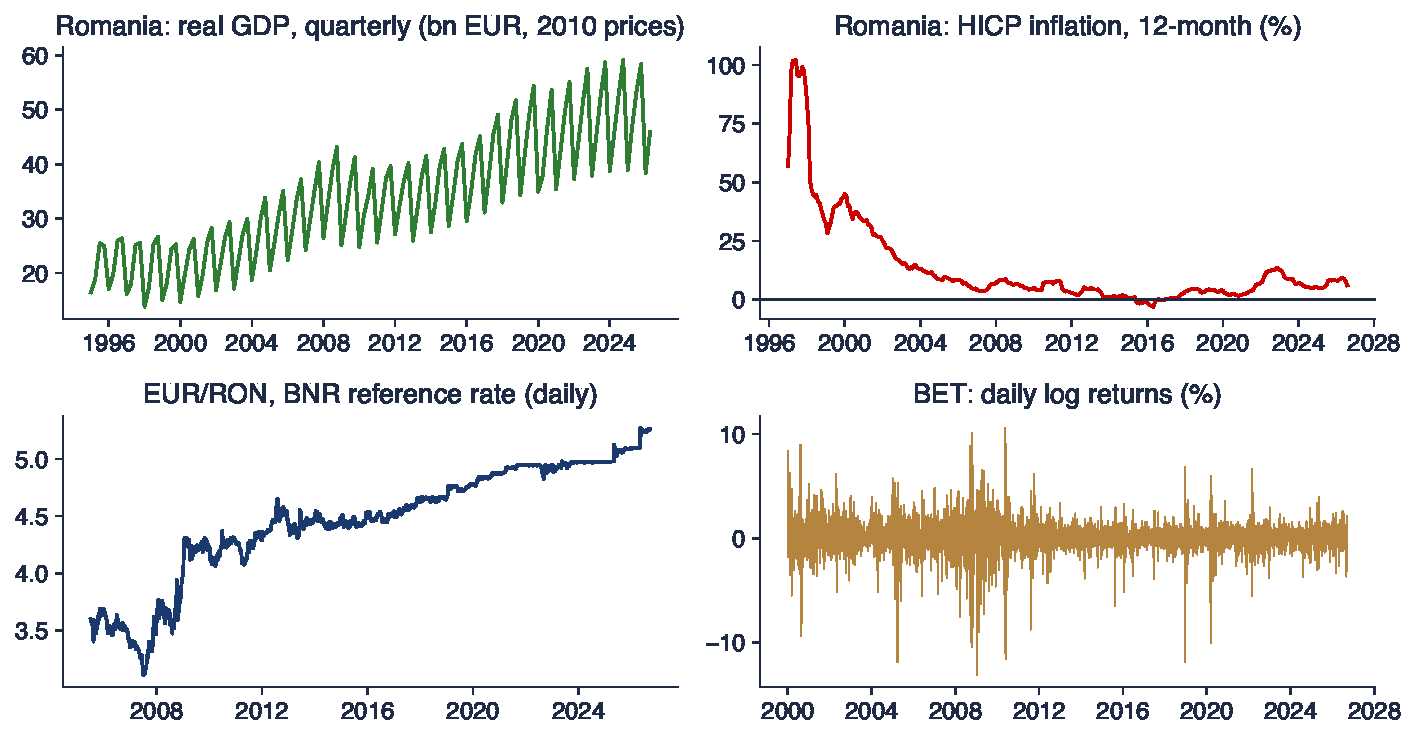
\includegraphics[width=0.97\textwidth,height=0.66\textheight,keepaspectratio]{tsa_ch1_four_series.pdf}
\end{center}
\vspace{-0.25cm}
\begin{itemize}
    \item PIB-ul real al României, T1 1995--T2 2026 (Eurostat); inflația IAPC (Eurostat); cursul EUR/RON, cursul de referință BNR; randamentele logaritmice zilnice ale BET din 2000
    \item Patru frecvențe (trimestrială, lunară, zilnică) și patru tipuri de comportament
\end{itemize}
\quantlet{TSA\_ch1\_real\_series}{\qlurl{TSA_ch1_real_series}}
\end{frame}

\begin{frame}{Interpretarea celor patru serii}
\itemsize{\small}
\begin{itemize}
    \item \textbf{PIB}: de la 16{,}5 la 45{,}9 mld. EUR pe trimestru; un trend și o sezonalitate a cărei amplitudine crește odată cu nivelul
    \begin{itemize}
        \item media seriei se schimbă în timp
    \end{itemize}
    \item \textbf{Inflația}: 102\% în iunie 1997, -3{,}0\% în mai 2016, 6{,}1\% în august 2026
    \begin{itemize}
        \item o mișcare lentă, persistentă: luna aceasta seamănă cu luna trecută
    \end{itemize}
    \item \textbf{EUR/RON}: de la 3{,}60 la 5{,}26 lei; rătăcește fără să revină la un nivel fix
    \begin{itemize}
        \item un candidat pentru un mers aleator (secțiunea 3)
    \end{itemize}
    \item \textbf{Randamentele BET}: oscilează în jurul unui nivel constant, apropiat de 0; extremele: $-13{,}1\%$ pe 7 ianuarie 2009, $+10{,}6\%$ pe 10 mai 2010
    \begin{itemize}
        \item dar amplitudinea se schimbă: abaterea standard este 3{,}62\% în septembrie 2008--martie 2009 și 0{,}66\% în 2017
    \end{itemize}
\end{itemize}
\end{frame}

\begin{frame}{Seria de timp ca o realizare}
\itemsize{\small}
\begin{itemize}
    \item \textbf{Serie de timp}: observații $x_1, x_2, \dots, x_T$ ordonate în timp, la intervale egale
    \begin{itemize}
        \item $T$ = volumul eșantionului; $t$ = indicele de timp (zi, lună, trimestru)
    \end{itemize}
    \item Ideea de bază: fiecare $x_t$ este valoarea observată a unei \textbf{variabile aleatoare} $X_t$
    \begin{itemize}
        \item randamentul BET de mîine este necunoscut azi: are o distribuție de valori posibile
        \item istoria s-a desfășurat o singură dată: vedem cîte o singură valoare din fiecare distribuție
    \end{itemize}
    \item Consecința: avem nevoie de ipoteze care leagă distribuțiile de la date diferite
    \begin{itemize}
        \item altfel, $T$ observații ar estima $T$ medii diferite
    \end{itemize}
\end{itemize}
\end{frame}

\begin{frame}{Procesul stochastic}
\itemsize{\small}
\begin{itemize}
    \item \textbf{Definiție}: un \textbf{proces stochastic} este o familie de variabile aleatoare $\{X_t : t \in \mathcal{T}\}$ definite pe același spațiu de probabilitate $(\Omega, \mathcal{F}, P)$
    \begin{itemize}
        \item $\mathcal{T} = \mathbb{Z}$ sau $\{1, \dots, T\}$: \textbf{timp discret}, cazul acestui curs
        \item $\Omega$: mulțimea „istoriilor” posibile $\omega$; $P$: probabilitățile lor
    \end{itemize}
    \item Două moduri de a privi $X_t(\omega)$
    \begin{itemize}
        \item fixăm $t$: $X_t$ este o variabilă aleatoare (toate valorile posibile la data $t$)
        \item fixăm $\omega$: $t \mapsto X_t(\omega)$ este o \textbf{traiectorie} (realizare): ceea ce observăm
    \end{itemize}
    \item Procesul este descris de \textbf{distribuțiile finit-dimensionale}: distribuția comună a lui $(X_{t_1}, \dots, X_{t_k})$ pentru orice date $t_1, \dots, t_k$
\end{itemize}
\end{frame}

\begin{frame}{Un ansamblu de traiectorii}
\itemsize{\footnotesize}
\begin{center}
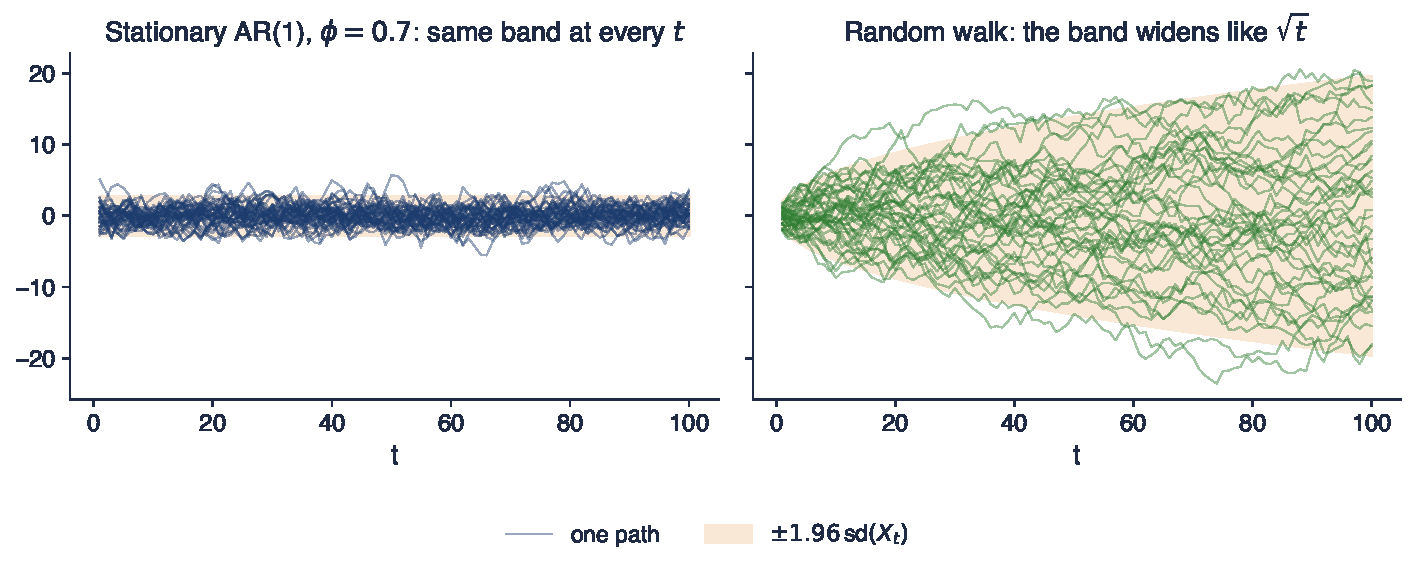
\includegraphics[width=0.97\textwidth,height=0.64\textheight,keepaspectratio]{tsa_ch1_ensemble.pdf}
\end{center}
\vspace{-0.25cm}
\begin{itemize}
    \item Stînga: 40 de traiectorii ale lui $X_t = 0{,}7X_{t-1} + \varepsilon_t$, $\varepsilon_t \sim N(0, 1)$ i.i.d. (independente și identic distribuite); dreapta: 40 de traiectorii ale lui $X_t = X_{t-1} + \varepsilon_t$, $X_0 = 0$
    \item Banda colorată: $\pm 1{,}96$ abateri standard ale lui $X_t$ la fiecare $t$
\end{itemize}
\quantlet{TSA\_ch1\_processes}{\qlurl{TSA_ch1_processes}}
\end{frame}

\begin{frame}{Interpretarea ansamblului de traiectorii}
\itemsize{\small}
\begin{itemize}
    \item O secțiune verticală la data $t$ arată \textbf{distribuția lui $X_t$}; o traiectorie arată \textbf{o singură istorie}
    \begin{itemize}
        \item momentele procesului (media, varianța) sînt medii pe traiectorii, la $t$ fixat
    \end{itemize}
    \item Stînga: aceeași bandă la orice $t$: $\mathrm{Var}(X_t) = 1/(1 - 0{,}7^2) = 1{,}96$, banda $\pm 2{,}74$
    \begin{itemize}
        \item distribuția lui $X_t$ nu depinde de $t$: o primă imagine a \textbf{staționarității}
    \end{itemize}
    \item Dreapta: banda se lărgește; pe 5000 de traiectorii simulate, $\mathrm{Var}(X_{100}) = 100{,}8$ (teoretic: 100)
    \begin{itemize}
        \item distribuția se schimbă cu $t$: mersul aleator \textbf{nu este staționar}
    \end{itemize}
\end{itemize}
\end{frame}

\begin{frame}{Funcțiile de medie, autocovarianță și autocorelație}
\itemsize{\small}
\begin{itemize}
    \item Pentru un proces cu $E[X_t^2] < \infty$ pentru orice $t$:
    \begin{itemize}
        \item \textbf{funcția de medie}: $\mu_t = E[X_t]$
        \item \textbf{funcția de autocovarianță}: $\gamma(t, s) = \mathrm{Cov}(X_t, X_s) = E[(X_t - \mu_t)(X_s - \mu_s)]$
        \item \textbf{funcția de autocorelație}: $\rho(t, s) = \gamma(t, s)/\sqrt{\gamma(t, t)\,\gamma(s, s)}$
    \end{itemize}
    \item „Auto”: covarianța seriei cu ea însăși la două date
    \begin{itemize}
        \item $\gamma(t, t) = \mathrm{Var}(X_t)$; $\rho(t, t) = 1$; $|\rho(t, s)| \le 1$ (inegalitatea Cauchy--Schwarz)
    \end{itemize}
    \item \textbf{Exemplu}: $X_t = a + bt + \varepsilon_t$, $\varepsilon_t$ i.i.d. cu media 0 și varianța $\sigma^2$
    \begin{itemize}
        \item $\mu_t = a + bt$ depinde de $t$; $\gamma(t, t) = \sigma^2$, $\gamma(t, s) = 0$ pentru $t \ne s$
    \end{itemize}
\end{itemize}
\end{frame}

\begin{frame}{Recapitulare: serii de timp și procese stochastice}
\itemsize{\small}
\begin{itemize}
    \item O serie de timp este o traiectorie a unui proces stochastic $\{X_t\}$
    \item Momentele sînt medii pe traiectorii, la date fixate: $\mu_t$, $\gamma(t, s)$, $\rho(t, s)$
    \item Cu o singură traiectorie, trebuie să presupunem că aceste funcții nu se schimbă în timp
\end{itemize}
\end{frame}


%=============================================================================
\section{Staționaritate}
%=============================================================================

\begin{frame}{Staționaritatea strictă}
\itemsize{\small}
\begin{itemize}
    \item \textbf{Definiție}: $\{X_t\}$ este \textbf{strict staționar} dacă, pentru orice $k \ge 1$, orice date $t_1, \dots, t_k$ și orice deplasare $h$:
    \begin{itemize}
        \item $(X_{t_1}, \dots, X_{t_k}) \overset{d}{=} (X_{t_1 + h}, \dots, X_{t_k + h})$, unde $\overset{d}{=}$ înseamnă distribuții comune egale
    \end{itemize}
    \item Consecințe
    \begin{itemize}
        \item $k = 1$: toate variabilele $X_t$ au aceeași distribuție
        \item $k = 2$: distribuția comună a lui $(X_t, X_{t+h})$ depinde doar de decalajul $h$
    \end{itemize}
    \item Exemplu: un șir i.i.d. este strict staționar
    \begin{itemize}
        \item definiția privește distribuții întregi; momentele nici nu trebuie să existe (un șir i.i.d. Cauchy)
    \end{itemize}
    \item Greu de verificat din date: ar trebui cunoscute toate distribuțiile comune
\end{itemize}
\end{frame}

\begin{frame}{Staționaritatea slabă}
\itemsize{\small}
\begin{itemize}
    \item \textbf{Definiție} \refKhinchin: $\{X_t\}$ este \textbf{slab staționar} (staționar în covarianță, staționar de ordinul doi) dacă
    \begin{itemize}
        \item (i) $E[X_t^2] < \infty$ pentru orice $t$
        \item (ii) $E[X_t] = \mu$, aceeași pentru orice $t$
        \item (iii) $\mathrm{Cov}(X_t, X_{t+h}) = \gamma(h)$ depinde doar de decalajul $h$, nu de $t$
    \end{itemize}
    \item Atunci funcțiile au un singur argument, \textbf{decalajul} $h$:
    \begin{itemize}
        \item $\gamma(h) = \mathrm{Cov}(X_t, X_{t+h})$, $\gamma(0) = \mathrm{Var}(X_t)$
        \item $\rho(h) = \gamma(h)/\gamma(0)$: \textbf{ACF} (funcția de autocorelație)
    \end{itemize}
    \item În acest curs, „staționar” înseamnă slab staționar, dacă nu se precizează altfel
\end{itemize}
\end{frame}

\begin{frame}{Staționaritatea strictă și cea slabă}
\itemsize{\small}
\begin{itemize}
    \item \textbf{Strictă + varianță finită $\Rightarrow$ slabă}
    \begin{itemize}
        \item distribuții egale dau medii egale; distribuții comune egale ale lui $(X_t, X_{t+h})$ dau covarianțe egale
    \end{itemize}
    \item \textbf{Slabă $\not\Rightarrow$ strictă}
    \begin{itemize}
        \item staționaritatea slabă fixează doar primele două momente; forma distribuției se poate schimba (slide-ul următor)
    \end{itemize}
    \item \textbf{Strictă $\not\Rightarrow$ slabă} dacă varianța este infinită
    \begin{itemize}
        \item șir i.i.d. Student-t cu 2 grade de libertate: strict staționar, fără varianță finită
    \end{itemize}
    \item \textbf{Procese gaussiene}: toate distribuțiile finit-dimensionale sînt Normale multivariate
    \begin{itemize}
        \item o distribuție Normală este determinată de medii și covarianțe, deci pentru ele slabă $\Leftrightarrow$ strictă
    \end{itemize}
\end{itemize}
\end{frame}

\begin{frame}{Slab, dar nu strict staționar}
\itemsize{\footnotesize}
\begin{center}
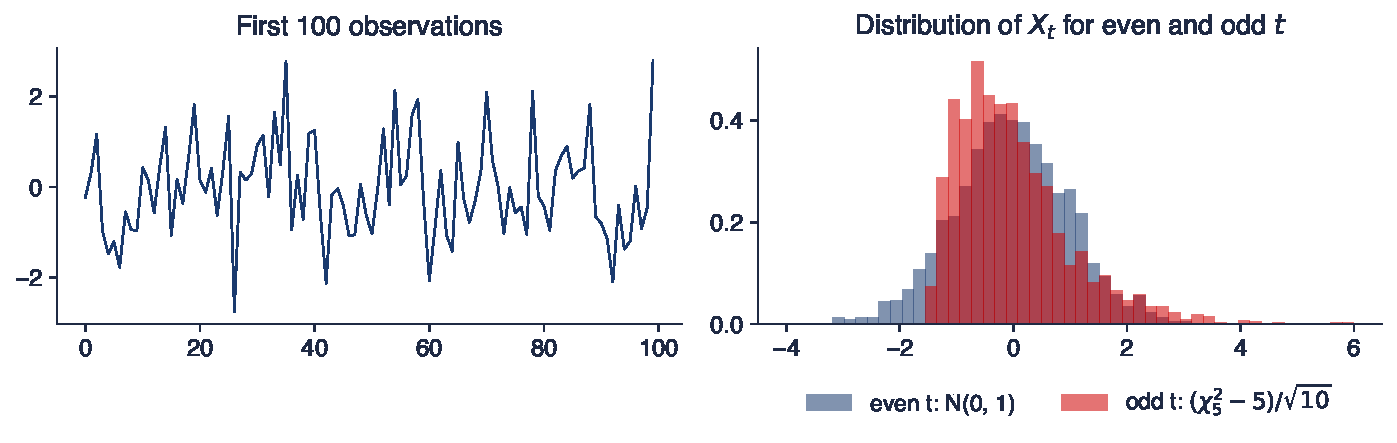
\includegraphics[width=0.97\textwidth,height=0.60\textheight,keepaspectratio]{tsa_ch1_counterexample.pdf}
\end{center}
\vspace{-0.25cm}
\begin{itemize}
    \item $X_t$ independente: $N(0, 1)$ pentru $t$ par, $(\chi^2_5 - 5)/\sqrt{10}$ pentru $t$ impar; ambele au media 0 și varianța 1
    \item Eșantion de 4000: varianța 0{,}99 (par) și 1{,}00 (impar); asimetria $-0{,}02$ și $1{,}30$ (teoretic: 0 și 1{,}26)
\end{itemize}
\quantlet{TSA\_ch1\_processes}{\qlurl{TSA_ch1_processes}}
\end{frame}

\begin{frame}{Interpretarea contraexemplului}
\itemsize{\small}
\begin{itemize}
    \item Slab staționar: $E[X_t] = 0$, $\gamma(0) = 1$, $\gamma(h) = 0$ pentru $h \ne 0$, la orice $t$
    \begin{itemize}
        \item ACF nu poate deosebi acest proces de zgomotul alb gaussian
    \end{itemize}
    \item Nu este strict staționar: distribuția lui $X_t$ alternează între una simetrică și una asimetrică la dreapta
    \begin{itemize}
        \item $P(X_t < -1{,}6)$: circa 5\% pentru $t$ par, 0 pentru $t$ impar ($X_t \ge -5/\sqrt{10} = -1{,}58$)
    \end{itemize}
    \item Lecția: momentele de ordinul doi rezumă dependența, dar nu întreaga distribuție; riscul din cozi cere mai mult (\tsachlink{https://danpele.github.io/Time-Series-Analysis/RO/Cursuri/capitol5_volatilitate_conditionata_garch.pdf}{Capitolul 5})
\end{itemize}
\end{frame}

\begin{frame}{Proprietățile funcției de autocovarianță}
\itemsize{\small}
\begin{itemize}
    \item Pentru un proces slab staționar:
    \begin{itemize}
        \item \textbf{simetrie}: $\gamma(-h) = \gamma(h)$, deoarece $\mathrm{Cov}(X_t, X_{t-h}) = \mathrm{Cov}(X_{t-h}, X_t)$
        \item \textbf{mărginire}: $|\gamma(h)| \le \gamma(0)$, deci $|\rho(h)| \le 1$
        \item \textbf{pozitiv semidefinire}: $\sum_{i,j} a_i a_j \gamma(i - j) \ge 0$ pentru orice numere reale $a_1, \dots, a_n$
    \end{itemize}
    \item Demonstrația celei de-a treia proprietăți
    \begin{itemize}
        \item $0 \le \mathrm{Var}\big(\sum_i a_i X_i\big) = \sum_{i,j} a_i a_j \mathrm{Cov}(X_i, X_j) = \sum_{i,j} a_i a_j \gamma(i - j)$
    \end{itemize}
    \item Consecință: nu orice șir este o ACF
    \begin{itemize}
        \item $\rho(1) = 0{,}9$, $\rho(2) = -0{,}9$ este imposibil: cu $a = (1, -1, -1)$, $\mathrm{Var}(X_1 - X_2 - X_3) = \gamma(0)(3 - 2\rho(1) - 2\rho(1) + 2\rho(2)) < 0$
    \end{itemize}
\end{itemize}
\end{frame}

\begin{frame}{Exemplu rezolvat: o medie mobilă de ordinul 1}
\itemsize{\small}
\begin{itemize}
    \item $X_t = \varepsilon_t + \theta\varepsilon_{t-1}$, $\{\varepsilon_t\}$ necorelate, media 0, varianța $\sigma^2$: procesul \textbf{MA(1)} (medie mobilă)
    \begin{itemize}
        \item media: $E[X_t] = 0$
        \item $\gamma(0) = E[(\varepsilon_t + \theta\varepsilon_{t-1})^2] = \sigma^2(1 + \theta^2)$ (termenul încrucișat are media 0)
        \item $\gamma(1) = E[(\varepsilon_t + \theta\varepsilon_{t-1})(\varepsilon_{t+1} + \theta\varepsilon_t)] = \theta\sigma^2$
        \item $\gamma(h) = 0$ pentru $|h| \ge 2$: nu există niciun șoc comun
    \end{itemize}
    \item Niciuna nu depinde de $t$: MA(1) este slab staționar pentru orice $\theta$
    \begin{itemize}
        \item $\rho(1) = \theta/(1 + \theta^2)$; cu $\theta = 0{,}6$, $\sigma^2 = 1$: $\gamma(0) = 1{,}36$, $\rho(1) = 0{,}441$
        \item $|\rho(1)| \le 0{,}5$ pentru orice $\theta$ (maximul la $\theta = 1$)
    \end{itemize}
\end{itemize}
\end{frame}

\begin{frame}{Exemplu rezolvat: o autoregresie de ordinul 1}
\itemsize{\small}
\begin{itemize}
    \item $X_t = \phi X_{t-1} + \varepsilon_t$, $|\phi| < 1$: procesul \textbf{AR(1)} (autoregresiv); presupunem că este staționar și aflăm momentele
    \begin{itemize}
        \item media: $\mu = \phi\mu + 0$, deci $\mu = 0$
        \item varianța: $\gamma(0) = \phi^2\gamma(0) + \sigma^2$, deci $\gamma(0) = \sigma^2/(1 - \phi^2)$
        \item înmulțim cu $X_{t-h}$ și aplicăm media: $\gamma(h) = \phi\gamma(h - 1)$, deci $\rho(h) = \phi^{|h|}$
    \end{itemize}
    \item Valori: $\phi = 0{,}8$, $\sigma^2 = 1$
    \begin{itemize}
        \item $\gamma(0) = 2{,}78$; $\rho(1) = 0{,}8$, $\rho(5) = 0{,}328$, $\rho(10) = 0{,}107$: descreștere geometrică
    \end{itemize}
    \item Cu $|\phi| \ge 1$ formula varianței nu mai funcționează: nu există o soluție staționară de această formă (\tsachlink{https://danpele.github.io/Time-Series-Analysis/RO/Cursuri/capitol2_modele_arma.pdf}{Capitolele 2}--\tsachlink{https://danpele.github.io/Time-Series-Analysis/RO/Cursuri/capitol3_radacini_unitare_modele_arima.pdf}{3})
\end{itemize}
\end{frame}

\begin{frame}{Întrebare pentru sală: care serii sînt staționare?}
\itemsize{\footnotesize}
\begin{center}
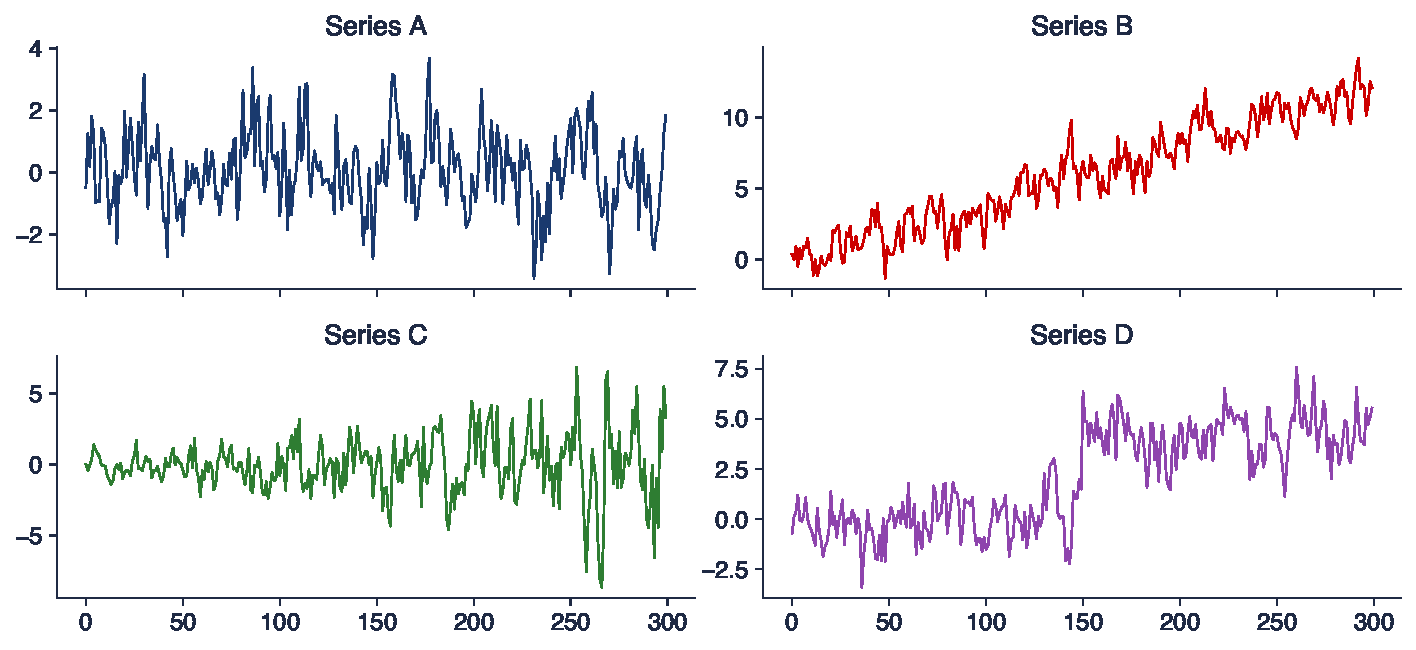
\includegraphics[width=0.97\textwidth,height=0.64\textheight,keepaspectratio]{tsa_ch1_nonstationary.pdf}
\end{center}
\vspace{-0.25cm}
\begin{itemize}
    \item Patru serii simulate, cu cîte 300 de observații; la baza tuturor stă același tip de zgomot AR(1) cu $\phi = 0{,}5$
    \item Care dintre condițiile (ii) și (iii) ale staționarității slabe nu este îndeplinită pentru fiecare serie?
\end{itemize}
\quantlet{TSA\_ch1\_processes}{\qlurl{TSA_ch1_processes}}
\end{frame}

\begin{frame}{Răspuns: doar seria A este staționară}
\itemsize{\small}
\begin{itemize}
    \item \textbf{A}: AR(1) staționar: media și varianța constante, ACF depinde doar de decalaj
    \item \textbf{B}: trend determinist, $\mu_t = 0{,}04\,t$: condiția (ii) nu este îndeplinită
    \begin{itemize}
        \item o serie \textbf{staționară în jurul trendului}: staționară în jurul unei drepte, după eliminarea trendului
    \end{itemize}
    \item \textbf{C}: abaterea standard crește de 7{,}5 ori de-a lungul eșantionului: condiția (iii) nu este îndeplinită la $h = 0$
    \item \textbf{D}: un salt de nivel de $+4$ la $t = 150$: condiția (ii) nu este îndeplinită
    \begin{itemize}
        \item o ruptură structurală; în date reale: o schimbare de regim sau de politică (Nilul, secțiunea 8)
    \end{itemize}
    \item În practică, graficul seriei este prima verificare; testele formale apar în \tsachlink{https://danpele.github.io/Time-Series-Analysis/RO/Cursuri/capitol3_radacini_unitare_modele_arima.pdf}{Capitolul 3}
\end{itemize}
\end{frame}

\begin{frame}{Recapitulare: staționaritate}
\itemsize{\small}
\begin{itemize}
    \item Strictă: toate distribuțiile comune sînt invariante la deplasare; slabă: media constantă, $\gamma$ depinde doar de decalaj
    \item Strictă + varianță finită $\Rightarrow$ slabă; pentru procesele gaussiene coincid
    \item MA(1) este întotdeauna staționar; AR(1) este staționar pentru $|\phi| < 1$, cu $\rho(h) = \phi^{|h|}$
    \item Trendurile, varianța variabilă și rupturile încalcă staționaritatea
\end{itemize}
\end{frame}


%=============================================================================
\section{Zgomotul alb și mersul aleator}
%=============================================================================

\begin{frame}{Zgomotul alb}
\itemsize{\small}
\begin{itemize}
    \item \textbf{Definiție}: $\{\varepsilon_t\}$ este \textbf{zgomot alb}, $\varepsilon_t \sim \mathrm{WN}(0, \sigma^2)$, dacă
    \begin{itemize}
        \item $E[\varepsilon_t] = 0$, $\mathrm{Var}(\varepsilon_t) = \sigma^2$ și $\mathrm{Cov}(\varepsilon_t, \varepsilon_s) = 0$ pentru $t \ne s$
        \item deci $\rho(0) = 1$ și $\rho(h) = 0$ pentru orice $h \ne 0$
    \end{itemize}
    \item Trei variante, de la cea mai slabă la cea mai tare
    \begin{itemize}
        \item zgomot alb \textbf{slab}: doar necorelat; dependența neliniară este permisă (de exemplu, în pătrate)
        \item zgomot alb \textbf{i.i.d.} (tare): independent și identic distribuit
        \item zgomot alb \textbf{gaussian}: i.i.d. $N(0, \sigma^2)$; pentru variabile comun Normale, necorelat înseamnă independent
    \end{itemize}
    \item Zgomotul alb este piesa de bază a tuturor modelelor din acest curs: ARMA, ARIMA, GARCH, VAR
\end{itemize}
\end{frame}

\begin{frame}{Trei tipuri de zgomot alb}
\itemsize{\footnotesize}
\begin{center}
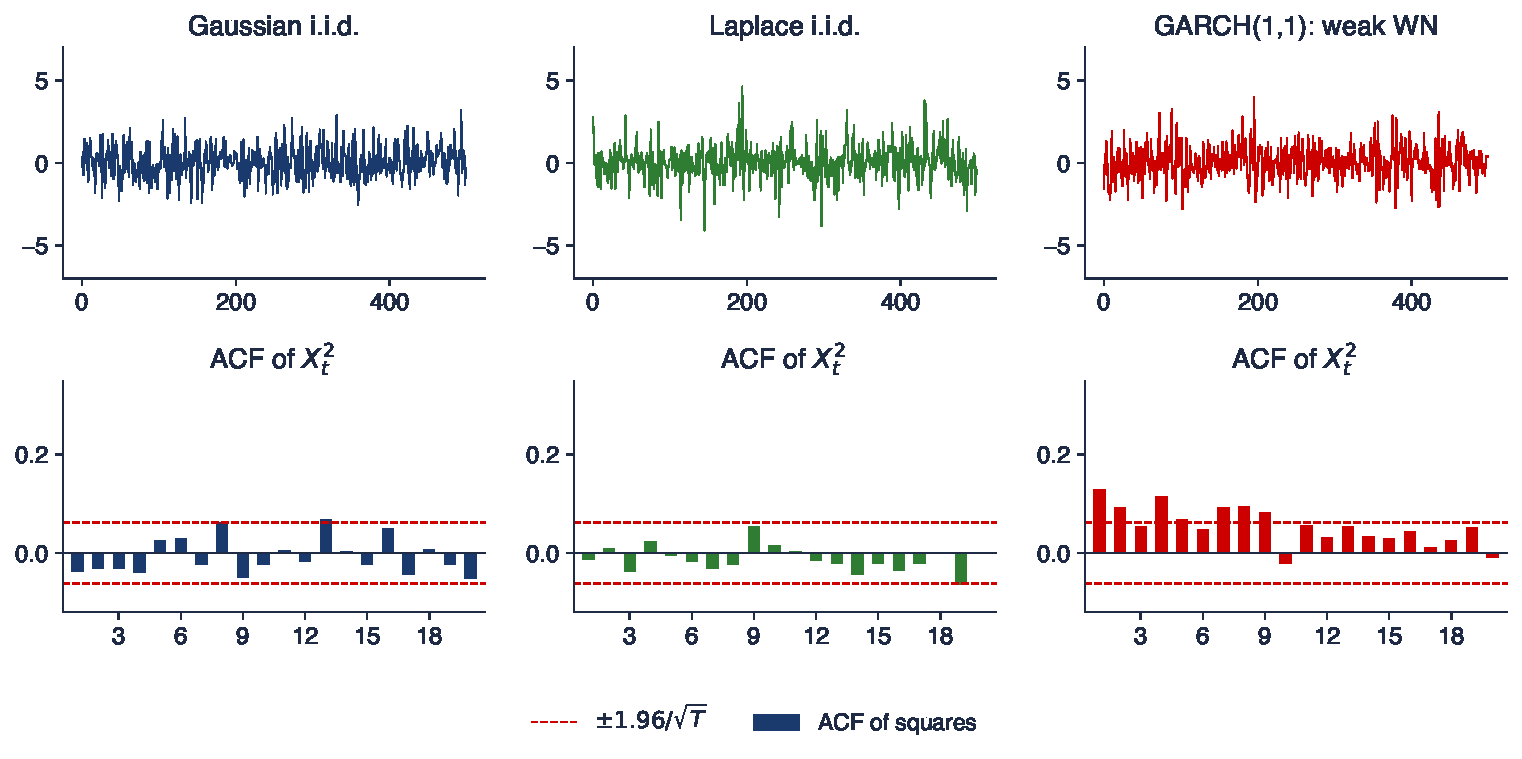
\includegraphics[width=0.97\textwidth,height=0.64\textheight,keepaspectratio]{tsa_ch1_white_noise.pdf}
\end{center}
\vspace{-0.25cm}
\begin{itemize}
    \item Sus: 500 din cele 1000 de valori simulate, varianța 1 în toate trei; jos: ACF a pătratelor $X_t^2$
    \item GARCH(1,1) (\tsachlink{https://danpele.github.io/Time-Series-Analysis/RO/Cursuri/capitol5_volatilitate_conditionata_garch.pdf}{Capitolul 5}): $\sigma_t^2 = 0{,}05 + 0{,}10\,\varepsilon_{t-1}^2 + 0{,}85\,\sigma_{t-1}^2$, $\varepsilon_t = \sigma_t z_t$
\end{itemize}
\quantlet{TSA\_ch1\_processes}{\qlurl{TSA_ch1_processes}}
\end{frame}

\begin{frame}{Interpretarea celor trei zgomote albe}
\itemsize{\small}
\begin{itemize}
    \item Toate trei sînt zgomot alb prin construcție; testul Ljung--Box $Q^*(10)$ (secțiunea 6) pentru $X_t$: p = 0{,}278 (gaussian), 0{,}986 (Laplace), 0{,}049 (GARCH)
    \begin{itemize}
        \item seria GARCH este aproape de respingere, deși este necorelată: cînd varianța se schimbă, testul obișnuit respinge prea des
    \end{itemize}
    \item Laplace: cozi mai groase (coeficientul de boltire 5{,}2, față de 3{,}0), dar tot i.i.d.: pătratele sînt necorelate (p = 0{,}680)
    \begin{itemize}
        \item cozile groase singure nu creează dependență
    \end{itemize}
    \item GARCH: pătratele sînt puternic corelate, $Q^*(10) = 73{,}2$, p $<$\,0{,}001
    \begin{itemize}
        \item un zgomot alb slab: semnul și nivelul nu pot fi anticipate, mărimea poate fi (volatility clustering)
        \item randamentele zilnice se comportă așa (BET, secțiunea 5)
    \end{itemize}
\end{itemize}
\end{frame}

\begin{frame}{Mersul aleator}
\itemsize{\small}
\begin{itemize}
    \item \textbf{Definiție}: $X_t = X_{t-1} + \varepsilon_t$, $t \ge 1$, $X_0 = 0$, $\varepsilon_t \sim \mathrm{WN}(0, \sigma^2)$; prin substituție, $X_t = \sum_{i=1}^{t}\varepsilon_i$
    \begin{itemize}
        \item fiecare șoc rămîne pentru totdeauna în nivel: $\partial X_{t+h}/\partial\varepsilon_t = 1$ pentru orice $h \ge 0$
    \end{itemize}
    \item Momentele (sînt suficiente șocuri necorelate)
    \begin{itemize}
        \item $E[X_t] = 0$; $\mathrm{Var}(X_t) = \sum_{i=1}^{t}\mathrm{Var}(\varepsilon_i) = t\sigma^2$
        \item pentru $t \le s$: $\mathrm{Cov}(X_t, X_s) = \mathrm{Cov}\big(\sum_{i \le t}\varepsilon_i, \sum_{j \le s}\varepsilon_j\big) = t\sigma^2$
        \item $\rho(t, s) = t/\sqrt{ts} = \sqrt{t/s}$
    \end{itemize}
    \item \textbf{Nestaționar}: varianța crește cu $t$, iar corelația depinde de $t$, nu doar de $s - t$
    \begin{itemize}
        \item exemplu: $\rho(X_{100}, X_{110}) = \sqrt{100/110} = 0{,}953$, dar $\rho(X_{10}, X_{20}) = \sqrt{0{,}5} = 0{,}707$
    \end{itemize}
\end{itemize}
\end{frame}

\begin{frame}{Mersuri aleatoare și varianța lor}
\itemsize{\footnotesize}
\begin{center}
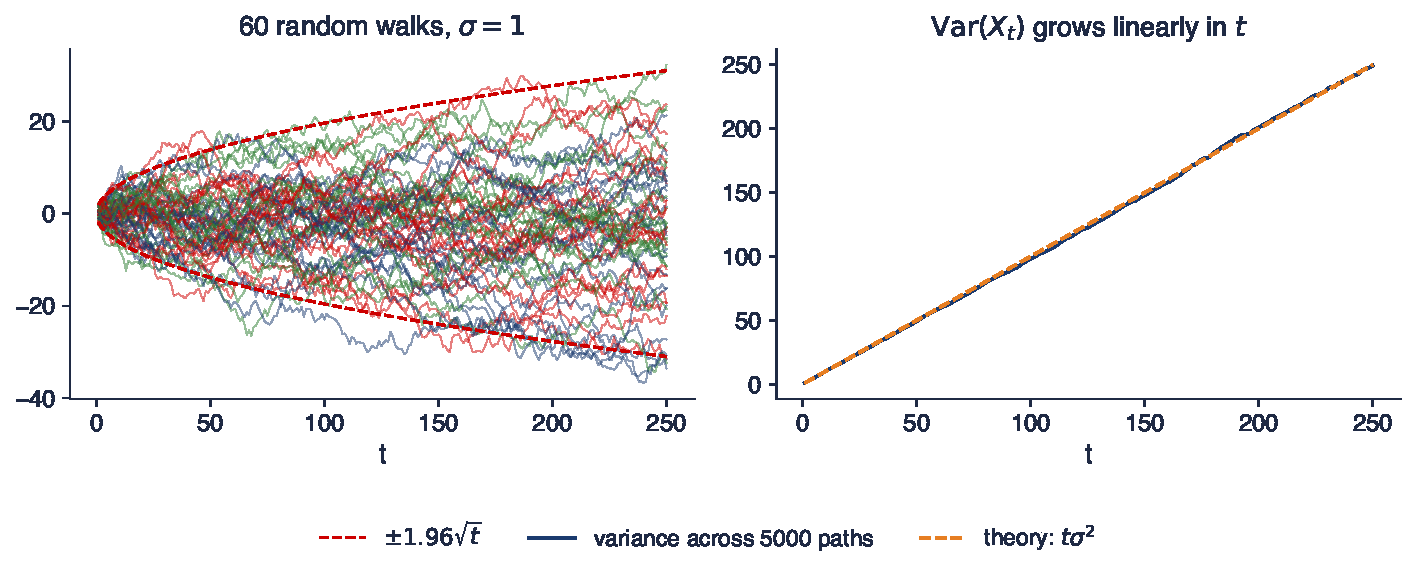
\includegraphics[width=0.97\textwidth,height=0.62\textheight,keepaspectratio]{tsa_ch1_random_walk.pdf}
\end{center}
\vspace{-0.25cm}
\begin{itemize}
    \item Stînga: 60 de traiectorii cu $\sigma = 1$ și banda $\pm 1{,}96\sqrt{t}$; dreapta: varianța lui $X_t$ pe 5000 de traiectorii și dreapta $t\sigma^2$
    \item La $t = 250$: varianța simulată 249{,}1 (teoretic: 250); proporția traiectoriilor în afara benzii: 5{,}0\%
\end{itemize}
\quantlet{TSA\_ch1\_processes}{\qlurl{TSA_ch1_processes}}
\end{frame}

\begin{frame}{Interpretarea mersurilor aleatoare}
\itemsize{\small}
\begin{itemize}
    \item Dispersia crește ca $\sqrt{t}$: incertitudinea despre nivel se acumulează
    \begin{itemize}
        \item o prognoză a nivelului peste 100 de zile are varianța $100\sigma^2$
    \end{itemize}
    \item Traiectoriile par să aibă trenduri și cicluri, deși nimic altceva decît hazardul nu le guvernează
    \begin{itemize}
        \item aceeași lecție ca la \refSlutzky: sumele de șocuri aleatoare pot semăna cu ciclurile economice
    \end{itemize}
    \item Valoarea simulată $\rho(X_{100}, X_{110}) = 0{,}953$, față de 0{,}953 teoretic
    \begin{itemize}
        \item nivelurile depărtate în timp rămîn puternic corelate: o ACF care scade foarte încet
    \end{itemize}
\end{itemize}
\end{frame}

\begin{frame}{Mersul aleator cu derivă}
\itemsize{\small}
\begin{itemize}
    \item $X_t = c + X_{t-1} + \varepsilon_t$, $X_0 = 0$: $X_t = ct + \sum_{i=1}^{t}\varepsilon_i$; $c$ este \textbf{deriva}
    \begin{itemize}
        \item $E[X_t] = ct$: un trend liniar în medie; $\mathrm{Var}(X_t) = t\sigma^2$, ca înainte
    \end{itemize}
    \item Prima diferență este staționară: $\Delta X_t = X_t - X_{t-1} = c + \varepsilon_t$
    \begin{itemize}
        \item o serie \textbf{staționară în diferențe}, cu \textbf{trend stochastic}
    \end{itemize}
    \item Comparație cu seria staționară în jurul trendului $Y_t = a + bt + u_t$, $u_t$ staționar
    \begin{itemize}
        \item ambele au o medie liniară; în $Y_t$ șocurile se sting, în $X_t$ rămîn pentru totdeauna
        \item deosebirea celor două este problema rădăcinii unitare din \tsachlink{https://danpele.github.io/Time-Series-Analysis/RO/Cursuri/capitol3_radacini_unitare_modele_arima.pdf}{Capitolul 3}
    \end{itemize}
    \item Logaritmii prețurilor acțiunilor și ai indicilor sînt adesea apropiați de un mers aleator cu o derivă mică și pozitivă
\end{itemize}
\end{frame}

\begin{frame}{Bursa de Valori București}
\itemsize{\small}
\begin{columns}[T]
\begin{column}{0.50\textwidth}
\centering

\includegraphics[height=0.50\textheight]{ch1_bvb_2024.jpg}\\[1mm]
\imgcap{Bursa de Valori București (BVB), 2024}
\imgcredit{https://commons.wikimedia.org/wiki/File:Bursa_de_Valori_București.jpg}{Foto: Corina Chitu (2024); CC BY-SA 4.0; Wikimedia Commons}
\end{column}
\begin{column}{0.46\textwidth}
\begin{itemize}
    \item Indicele BET: indicele de referință al BVB (Bursa de Valori București), calculat din 19 septembrie 1997
    \item Închideri zilnice din 2000: 6\,670 de randamente logaritmice $r_t = 100\,\Delta\ln P_t$; abaterea standard 1{,}40\% pe zi
    \item Este logaritmul prețului BET un mers aleator? Un prim test, vizual, pe slide-ul următor
\end{itemize}
\end{column}
\end{columns}
\end{frame}

\begin{frame}{Întrebare pentru sală: care serie este cea reală?}
\itemsize{\footnotesize}
\begin{center}
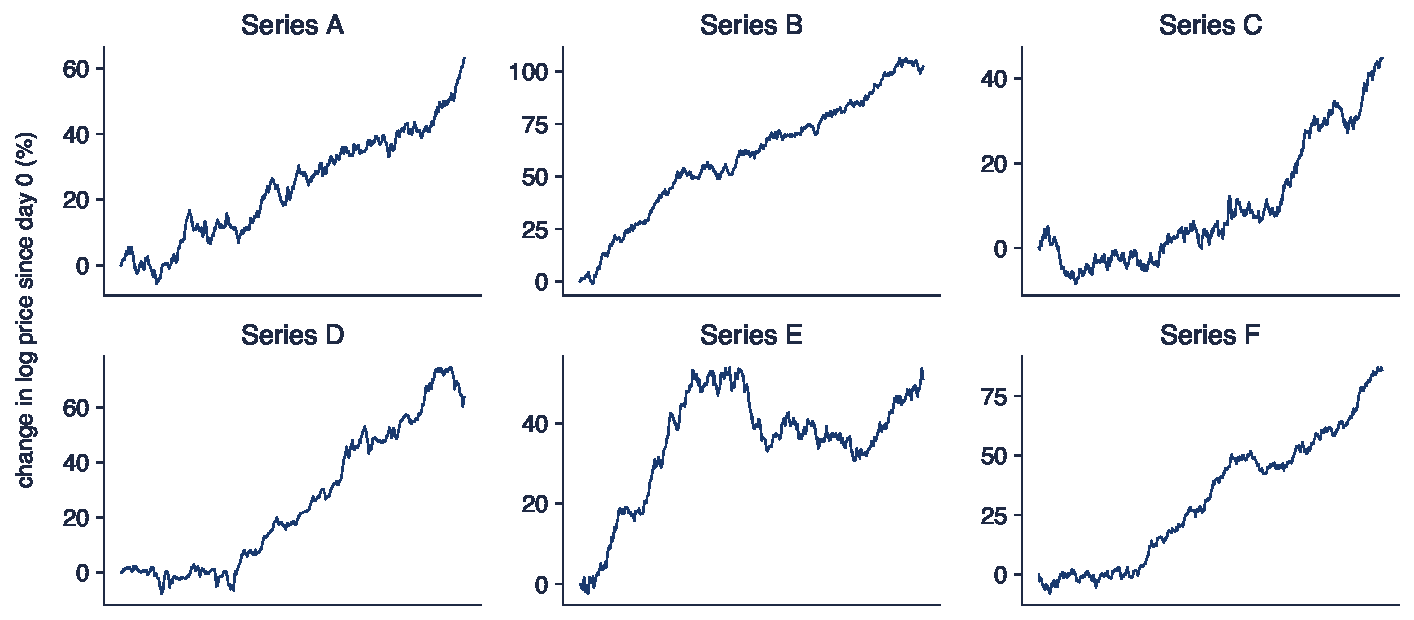
\includegraphics[width=0.97\textwidth,height=0.64\textheight,keepaspectratio]{tsa_ch1_spot_real.pdf}
\end{center}
\vspace{-0.25cm}
\begin{itemize}
    \item Un panou: logaritmul prețului BET în ultimele 500 de zile de tranzacționare; cinci panouri: mersuri aleatoare cu aceeași derivă și aceeași abatere standard zilnică
    \item Care panou este BET?
\end{itemize}
\quantlet{TSA\_ch1\_processes}{\qlurl{TSA_ch1_processes}}
\end{frame}

\begin{frame}{Răspuns: seria D}
\itemsize{\small}
\begin{itemize}
    \item Seria D este BET, 11 septembrie 2024--18 septembrie 2026: variația zilnică medie 0{,}13\%, abaterea standard 0{,}99\%
    \begin{itemize}
        \item cu ochiul liber, nu poate fi deosebită de mersurile aleatoare
    \end{itemize}
    \item Datele nu sînt exact un mers aleator: autocorelația de ordinul 1 a variațiilor zilnice este 0{,}12; valoarea p a testului Ljung--Box $Q^*(10)$ este 0{,}018
    \begin{itemize}
        \item abaterile mici, invizibile în nivel, apar în ACF a diferențelor
    \end{itemize}
    \item Lecția: studiem variațiile, nu nivelul; instrumentele sînt ACF și testele portmanteau (secțiunile 5--6)
\end{itemize}
\end{frame}

\begin{frame}{Recapitulare: zgomotul alb și mersul aleator}
\itemsize{\small}
\begin{itemize}
    \item Zgomotul alb: media 0, varianța constantă, fără autocorelație; slab, i.i.d. sau gaussian
    \item Necorelat nu înseamnă independent: pătratele unui zgomot alb slab pot fi corelate
    \item Mersul aleator: $\mathrm{Var}(X_t) = t\sigma^2$, $\rho(t, s) = \sqrt{t/s}$: nestaționar; diferența lui este zgomot alb
    \item Seriile staționare în jurul trendului și cele staționare în diferențe arată la fel, dar reacționează diferit la șocuri
\end{itemize}
\end{frame}


%=============================================================================
\section{Operatorul lag, diferențierea și descompunerea Wold}
%=============================================================================

\begin{frame}{Operatorul lag}
\itemsize{\small}
\begin{itemize}
    \item \textbf{Definiție}: $LX_t = X_{t-1}$; puteri: $L^kX_t = X_{t-k}$, $L^0 = 1$ (notat și $B$, operatorul de întîrziere)
    \begin{itemize}
        \item o constantă nu se schimbă: $Lc = c$
    \end{itemize}
    \item \textbf{Polinoame în lag}: $\phi(L) = 1 - \phi_1L - \dots - \phi_pL^p$
    \begin{itemize}
        \item AR(1): $(1 - \phi L)X_t = \varepsilon_t$; MA(1): $X_t = (1 + \theta L)\varepsilon_t$
        \item se înmulțesc ca polinoamele obișnuite: $(1 - L)(1 + L) = 1 - L^2$
    \end{itemize}
    \item \textbf{Inversare}: pentru $|\phi| < 1$, $(1 - \phi L)^{-1} = 1 + \phi L + \phi^2L^2 + \dots$ (o serie geometrică)
    \begin{itemize}
        \item deci AR(1) se scrie $X_t = \sum_{j \ge 0}\phi^j\varepsilon_{t-j}$: o medie mobilă infinită
    \end{itemize}
    \item Limbajul \tsachlink{https://danpele.github.io/Time-Series-Analysis/RO/Cursuri/capitol2_modele_arma.pdf}{Capitolelor 2}--\tsachlink{https://danpele.github.io/Time-Series-Analysis/RO/Cursuri/capitol4_sezonalitate_prognoza.pdf}{4}: modelele ARMA, ARIMA și SARIMA se scriu cu polinoame în lag
\end{itemize}
\end{frame}

\begin{frame}{Diferențierea}
\itemsize{\small}
\begin{itemize}
    \item \textbf{Prima diferență}: $\Delta X_t = (1 - L)X_t = X_t - X_{t-1}$; \textbf{a doua}: $\Delta^2X_t = (1 - L)^2X_t = X_t - 2X_{t-1} + X_{t-2}$
    \begin{itemize}
        \item \textbf{diferența sezonieră} cu perioada $s$: $\Delta_sX_t = (1 - L^s)X_t = X_t - X_{t-s}$ ($s = 4$ pentru trimestre, $s = 12$ pentru luni)
    \end{itemize}
    \item \textbf{Exemplu rezolvat}: $x = (10, 12, 15, 14, 18)$
    \begin{itemize}
        \item $\Delta x = (2, 3, -1, 4)$; $\Delta^2x = (1, -4, 5)$; fiecare diferențiere pierde o observație
    \end{itemize}
    \item Ce elimină diferențierea
    \begin{itemize}
        \item un trend liniar: $\Delta(a + bt) = b$; un trend pătratic necesită $\Delta^2$
        \item un mers aleator: $\Delta X_t = \varepsilon_t$; un tipar sezonier care se repetă exact: $\Delta_s$
    \end{itemize}
    \item \textbf{Proces integrat}: $X_t \sim I(d)$ dacă $\Delta^dX_t$ este staționar, iar $\Delta^{d-1}X_t$ nu este
    \begin{itemize}
        \item zgomotul alb este $I(0)$, mersul aleator este $I(1)$; testarea lui $d$: \tsachlink{https://danpele.github.io/Time-Series-Analysis/RO/Cursuri/capitol3_radacini_unitare_modele_arima.pdf}{Capitolul 3}
    \end{itemize}
\end{itemize}
\end{frame}

\begin{frame}{S\&P 500: nivelul și diferența lui}
\itemsize{\footnotesize}
\begin{center}
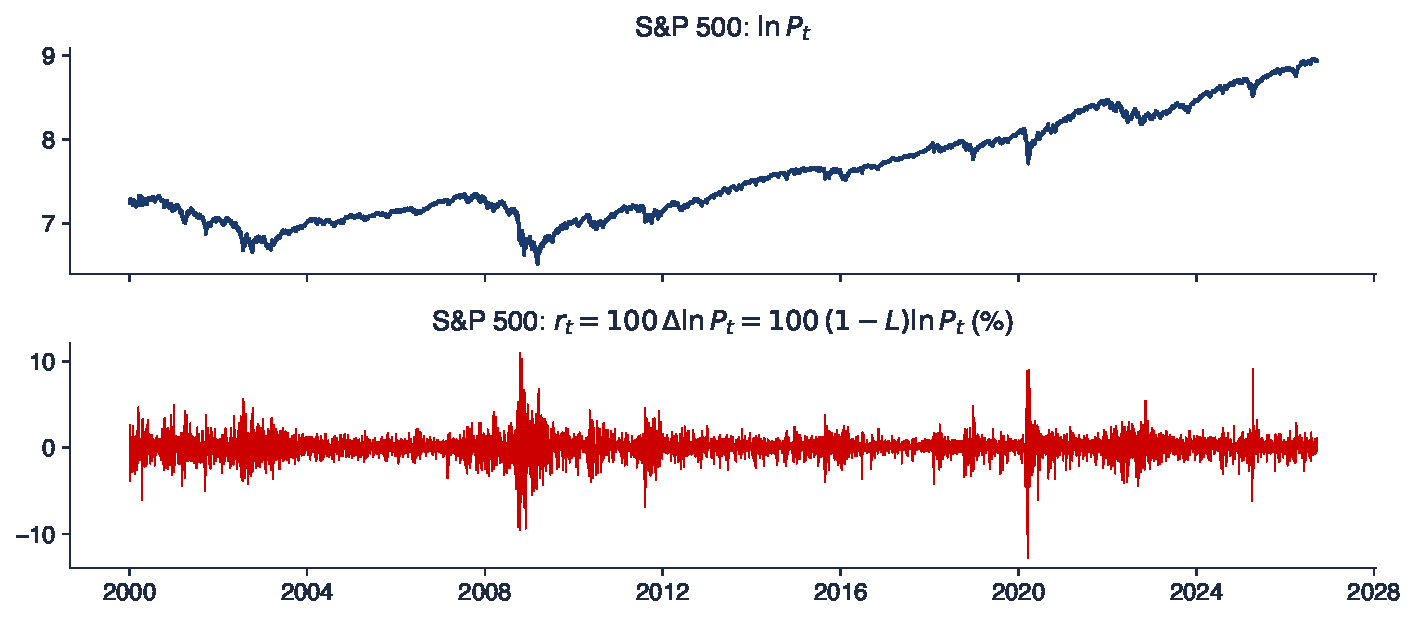
\includegraphics[width=0.97\textwidth,height=0.66\textheight,keepaspectratio]{tsa_ch1_sp500_diff.pdf}
\end{center}
\vspace{-0.25cm}
\begin{itemize}
    \item Sus: logaritmul indicelui S\&P 500 din 2000; jos: randamentele logaritmice zilnice, 6\,714 zile pînă la 18 septembrie 2026
\end{itemize}
\quantlet{TSA\_ch1\_transformations}{\qlurl{TSA_ch1_transformations}}
\end{frame}

\begin{frame}{Interpretarea transformării S\&P 500}
\itemsize{\small}
\begin{itemize}
    \item Logaritmul prețului: ACF de selecție 0{,}999 la decalajul 1 și încă 0{,}973 la decalajul 50
    \begin{itemize}
        \item comportamentul unui mers aleator: nivelul își amintește totul
    \end{itemize}
    \item Randamentele logaritmice: media 0{,}025\% pe zi, abaterea standard 1{,}21\%; ACF la decalajul 1: $-0{,}099$
    \begin{itemize}
        \item un nivel constant: o singură diferențiere a eliminat trendul stochastic
    \end{itemize}
    \item Nu încă zgomot alb în sens strict: perioadele liniștite alternează cu cele agitate (2008, 2020)
    \begin{itemize}
        \item randamentele sînt apropiate de un zgomot alb slab; varianța lor este subiectul \tsachlink{https://danpele.github.io/Time-Series-Analysis/RO/Cursuri/capitol5_volatilitate_conditionata_garch.pdf}{Capitolului 5}
    \end{itemize}
\end{itemize}
\end{frame}

\begin{frame}{Descompunerea Wold}
\itemsize{\footnotesize}
\begin{columns}[T]
\begin{column}{0.66\textwidth}
\begin{itemize}
    \item \textbf{Teoremă} \refWold: orice proces slab staționar cu media 0 se poate scrie
    \begin{itemize}
        \item $X_t = \sum_{j=0}^{\infty}\psi_j\varepsilon_{t-j} + \eta_t$, cu $\psi_0 = 1$, $\sum_j\psi_j^2 < \infty$
        \item $\varepsilon_t$: zgomot alb, eroarea celei mai bune prognoze liniare a lui $X_t$ din trecutul său (\textbf{inovația})
        \item $\eta_t$: o parte deterministă, perfect previzibilă din trecutul îndepărtat (de exemplu, un ciclu fix)
    \end{itemize}
    \item Semnificația
    \begin{itemize}
        \item orice serie staționară este o sumă ponderată de șocuri trecute: MA($\infty$)
        \item ponderile $\psi_j$ = efectul unui șoc după $j$ perioade (răspunsul la impuls)
        \item modelele ARMA (\tsachlink{https://danpele.github.io/Time-Series-Analysis/RO/Cursuri/capitol2_modele_arma.pdf}{Capitolul 2}) aproximează șirul infinit $\psi_j$ cu puțini parametri
    \end{itemize}
\end{itemize}
\end{column}
\begin{column}{0.30\textwidth}
\centering

\includegraphics[height=0.48\textheight]{ch1_herman_wold_1969.jpg}\\[1mm]
\imgcap{Herman Wold, Uppsala, 1969}
\imgcredit{https://commons.wikimedia.org/wiki/File:Professor_Herman_Wold,_Uppsala,_1969_(cropped).jpg}{Foto: Uppsala-Bild (1969); CC BY 4.0; Wikimedia Commons}
\end{column}
\end{columns}
\end{frame}

\begin{frame}{Ponderile Wold ale a patru procese}
\itemsize{\footnotesize}
\begin{center}
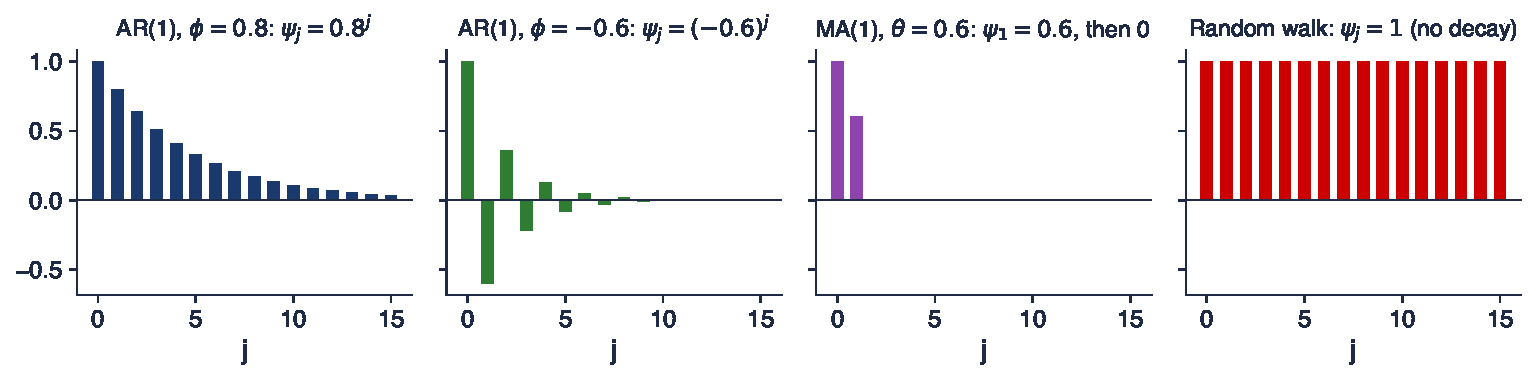
\includegraphics[width=0.97\textwidth,height=0.50\textheight,keepaspectratio]{tsa_ch1_wold.pdf}
\end{center}
\vspace{-0.25cm}
\begin{itemize}
    \item $\psi_j$, $j = 0, \dots, 15$: AR(1) cu $\phi = 0{,}8$ și $\phi = -0{,}6$, MA(1) cu $\theta = 0{,}6$ și mersul aleator
    \item AR(1), $\phi = 0{,}8$: $\psi_5 = 0{,}328$, $\psi_{10} = 0{,}107$; $\mathrm{Var}(X_t) = \sigma^2\sum_j\psi_j^2 = 2{,}78\,\sigma^2$
\end{itemize}
\quantlet{TSA\_ch1\_wold\_ergodicity}{\qlurl{TSA_ch1_wold_ergodicity}}
\end{frame}

\begin{frame}{Interpretarea ponderilor Wold}
\itemsize{\small}
\begin{itemize}
    \item Procesele staționare: $\psi_j \to 0$, deci șocurile se sting, iar varianța $\sigma^2\sum_j\psi_j^2$ este finită
    \begin{itemize}
        \item $\phi < 0$: efectul își schimbă semnul alternativ; MA(1): efectul se oprește după o perioadă
    \end{itemize}
    \item Mersul aleator: $\psi_j = 1$ pentru orice $j$, $\sum_j\psi_j^2 = \infty$: fără formă Wold, fără staționaritate
    \begin{itemize}
        \item sensul economic: un șoc permanent (un șoc tehnologic asupra PIB-ului, o știre în preț)
    \end{itemize}
    \item ACF este determinată de ponderi: $\gamma(h) = \sigma^2\sum_j\psi_j\psi_{j+h}$
\end{itemize}
\end{frame}

\begin{frame}{Ergodicitatea}
\itemsize{\small}
\begin{itemize}
    \item Staționaritatea spune că momentele sînt constante; mai trebuie să le estimăm dintr-o \textbf{singură} traiectorie
    \begin{itemize}
        \item media pe ansamblu: $\mu = E[X_t]$ (pe traiectorii); media în timp: $\bar X_T = \frac1T\sum_{t=1}^{T}X_t$ (de-a lungul unei traiectorii)
    \end{itemize}
    \item \textbf{Definiție}: un proces staționar este \textbf{ergodic pentru medie} dacă $\bar X_T \to \mu$ (în medie pătratică) cînd $T \to \infty$
    \begin{itemize}
        \item o condiție suficientă: $\gamma(h) \to 0$ cînd $h \to \infty$ (corelația dispare)
        \item dacă $\sum_h|\gamma(h)| < \infty$, atunci $T\,\mathrm{Var}(\bar X_T) \to \sum_{h=-\infty}^{\infty}\gamma(h)$
    \end{itemize}
    \item \textbf{Contraexemplu}: $X_t = Z + \varepsilon_t$, $Z \sim N(0, 1)$ extras o singură dată, $\varepsilon_t$ zgomot alb
    \begin{itemize}
        \item staționar, cu $\gamma(h) = 1$ pentru orice $h \ne 0$; $\bar X_T \to Z$, nu $\mu = 0$
    \end{itemize}
\end{itemize}
\end{frame}

\begin{frame}{Mediile în timp: proces ergodic și neergodic}
\itemsize{\footnotesize}
\begin{center}
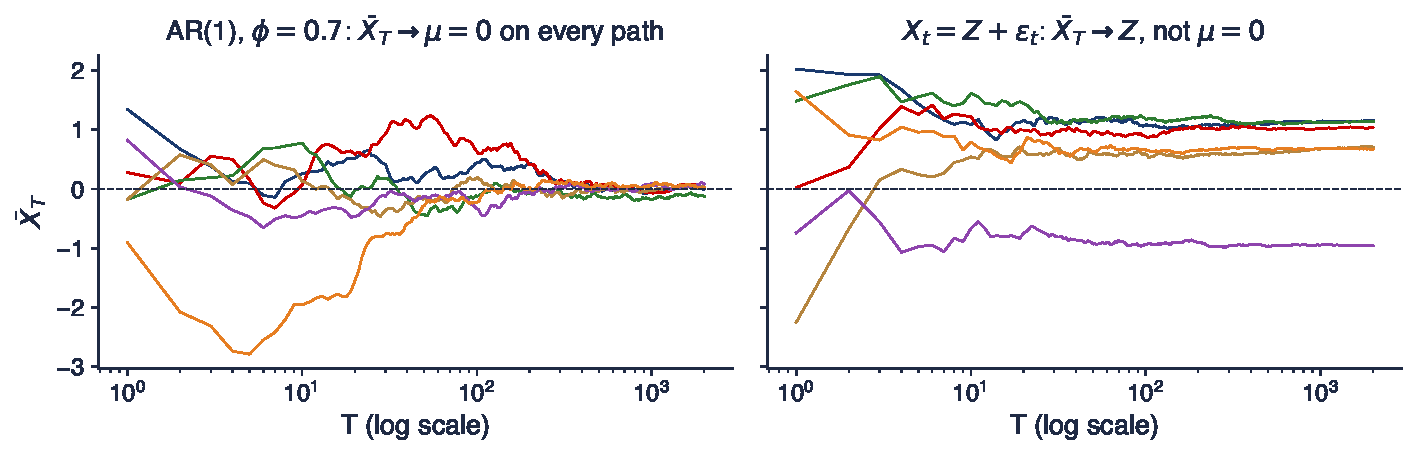
\includegraphics[width=0.97\textwidth,height=0.58\textheight,keepaspectratio]{tsa_ch1_ergodicity.pdf}
\end{center}
\vspace{-0.25cm}
\begin{itemize}
    \item Media cumulată $\bar X_T$ pe 6 traiectorii, $T$ pînă la 2\,000: AR(1) cu $\phi = 0{,}7$ (stînga) și $X_t = Z + \varepsilon_t$ (dreapta)
    \item Valorile finale: între $-0{,}13$ și $0{,}09$ în stînga; între $-0{,}95$ și $1{,}16$ în dreapta, aproape de $Z$ extras
\end{itemize}
\quantlet{TSA\_ch1\_wold\_ergodicity}{\qlurl{TSA_ch1_wold_ergodicity}}
\end{frame}

\begin{frame}{Interpretarea ergodicității}
\itemsize{\small}
\begin{itemize}
    \item Stînga: fiecare traiectorie „învață” media adevărată 0; o istorie lungă este la fel de bună ca multe istorii
    \begin{itemize}
        \item convergența este lentă cînd corelația este puternică: $\mathrm{Var}(\bar X_T) \approx \gamma(0)(1 + \phi)/((1 - \phi)T)$
    \end{itemize}
    \item Dreapta: fiecare traiectorie converge la propriul $Z$; oricîte date dintr-o singură traiectorie nu dezvăluie $\mu = 0$
    \begin{itemize}
        \item o economie cu un „tip” permanent și neobservat se comportă astfel
    \end{itemize}
    \item Ergodicitatea nu poate fi testată dintr-o singură traiectorie; o presupunem ori de cîte ori estimăm momente dintr-o singură serie
\end{itemize}
\end{frame}

\begin{frame}{Recapitulare: operatorul lag, diferențierea și descompunerea Wold}
\itemsize{\small}
\begin{itemize}
    \item $L^kX_t = X_{t-k}$; $\Delta = 1 - L$; $\Delta_s = 1 - L^s$; $I(d)$: staționar după $d$ diferențieri
    \item Wold: un proces staționar este un MA($\infty$) al inovațiilor sale, cu $\sum\psi_j^2 < \infty$
    \item Ergodicitatea permite ca mediile în timp să estimeze momentele pe ansamblu; cere corelații care se sting
\end{itemize}
\end{frame}


%=============================================================================
\section{ACF și PACF de selecție}
%=============================================================================

\begin{frame}{Autocovarianța și autocorelația de selecție}
\itemsize{\small}
\begin{itemize}
    \item Din $x_1, \dots, x_T$, cu media de selecție $\bar x = \frac1T\sum_t x_t$:
    \begin{itemize}
        \item $\hat\gamma(h) = \frac1T\sum_{t=1}^{T-h}(x_t - \bar x)(x_{t+h} - \bar x)$, $0 \le h < T$
        \item $\hat\rho(h) = \hat\gamma(h)/\hat\gamma(0)$: \textbf{ACF de selecție}; graficul lui $\hat\rho(h)$ în funcție de $h$ este \textbf{corelograma}
    \end{itemize}
    \item De ce împărțim la $T$ și nu la $T - h$?
    \begin{itemize}
        \item șirul $\hat\gamma(h)$ este atunci pozitiv semidefinit, ca o autocovarianță adevărată \refBD
        \item prețul: o mică deplasare spre 0 la decalaje mari; folosim $h \le T/4$
    \end{itemize}
    \item \textbf{Exemplu rezolvat}: $x = (3, 5, 4, 6, 7)$, $\bar x = 5$, abaterile $(-2, 0, -1, 1, 2)$
    \begin{itemize}
        \item $\hat\gamma(0) = 10/5 = 2{,}0$; $\hat\gamma(1) = (0 + 0 - 1 + 2)/5 = 0{,}2$; $\hat\gamma(2) = (2 + 0 - 2)/5 = 0{,}0$
        \item $\hat\rho(1) = 0{,}10$, $\hat\rho(2) = 0{,}00$; cu $T = 5$ banda este $\pm 0{,}88$: mult prea puține date
    \end{itemize}
\end{itemize}
\end{frame}

\begin{frame}{Benzi de încredere pentru ACF de selecție}
\itemsize{\small}
\begin{itemize}
    \item \textbf{Rezultatul asimptotic} din \refBartlett: dacă $X_t$ este i.i.d. cu varianță finită, pentru $T$ mare
    \begin{itemize}
        \item $\hat\rho(1), \dots, \hat\rho(m)$ sînt aproximativ independente, $N(0, 1/T)$
        \item banda de 95\%: $\pm 1{,}96/\sqrt{T}$; o bară în afara ei respinge $\rho(h) = 0$ la 5\%, \textbf{doar pentru acel decalaj}
    \end{itemize}
    \item Pentru un MA($q$), la decalaje $h > q$: $\mathrm{Var}(\hat\rho(h)) \approx \frac1T\big(1 + 2\sum_{k=1}^{q}\rho(k)^2\big)$
    \begin{itemize}
        \item benzile mai largi din \texttt{plot\_acf} din \texttt{statsmodels} (\tsachlink{https://danpele.github.io/Time-Series-Analysis/RO/Cursuri/capitol2_modele_arma.pdf}{Capitolul 2})
    \end{itemize}
    \item Două capcane
    \begin{itemize}
        \item cu 20 de decalaje și nicio corelație, ne așteptăm ca aproximativ o bară să iasă din bandă din întîmplare
        \item banda presupune date i.i.d.; pentru un zgomot alb slab (randamente GARCH) banda adevărată este mai largă
    \end{itemize}
\end{itemize}
\end{frame}

\begin{frame}{Distribuția de selecție a ACF}
\itemsize{\footnotesize}
\begin{center}
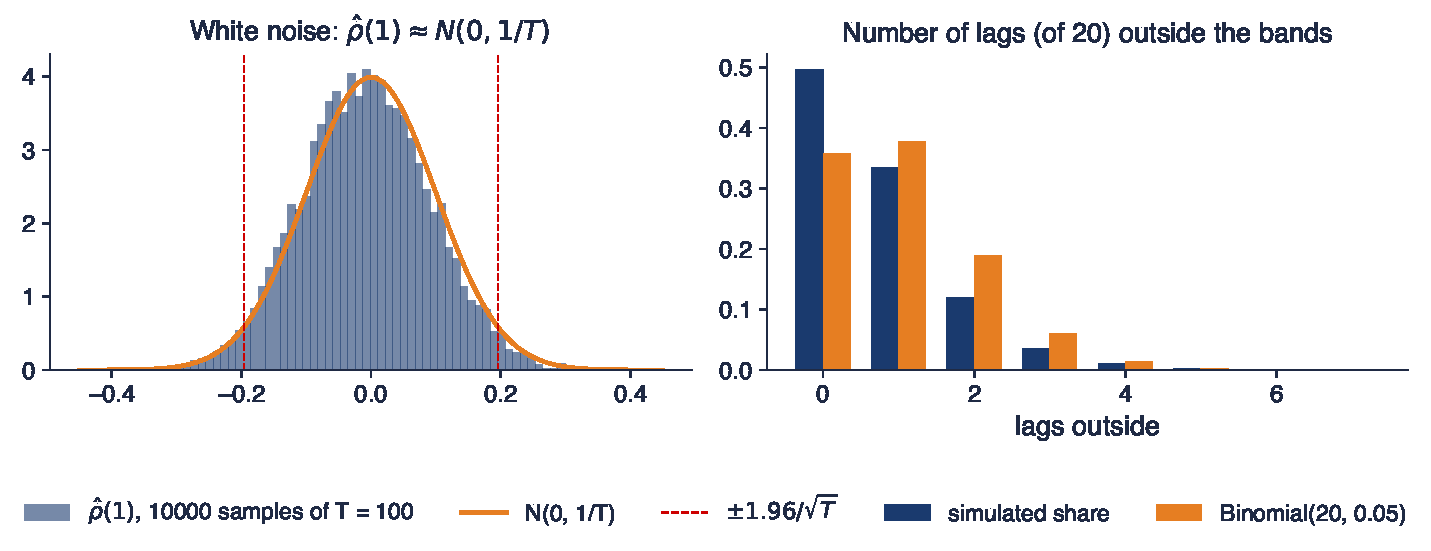
\includegraphics[width=0.97\textwidth,height=0.60\textheight,keepaspectratio]{tsa_ch1_bartlett.pdf}
\end{center}
\vspace{-0.25cm}
\begin{itemize}
    \item 10000 de eșantioane de zgomot alb gaussian cu $T = 100$: $\hat\rho(1)$ (stînga) și numărul de decalaje, din 20, în afara lui $\pm 0{,}196$ (dreapta)
\end{itemize}
\quantlet{TSA\_ch1\_acf\_pacf}{\qlurl{TSA_ch1_acf_pacf}}
\end{frame}

\begin{frame}{Interpretarea simulării}
\itemsize{\small}
\begin{itemize}
    \item $\hat\rho(1)$: media $-0{,}008$ (teoretic $-1/T = -0{,}01$), abaterea standard 0{,}098 (teoretic $1/\sqrt{T} = 0{,}1$)
    \begin{itemize}
        \item aproximarea lui Bartlett este deja bună la $T = 100$
    \end{itemize}
    \item Cel puțin una din 20 de bare iese din bandă în 50\% dintre eșantioane, deși nu există nicio corelație
    \begin{itemize}
        \item testele independente ar da $1 - 0{,}95^{20} = 64\%$; la decalaje mari $\mathrm{Var}(\hat\rho(h)) < 1/T$, deci ies ceva mai puține bare
    \end{itemize}
    \item Nu supra-interpretați bare izolate: judecați tiparul sau folosiți un test comun (secțiunea 6)
\end{itemize}
\end{frame}

\begin{frame}{ACF teoretică și de selecție pentru patru procese}
\itemsize{\footnotesize}
\begin{center}
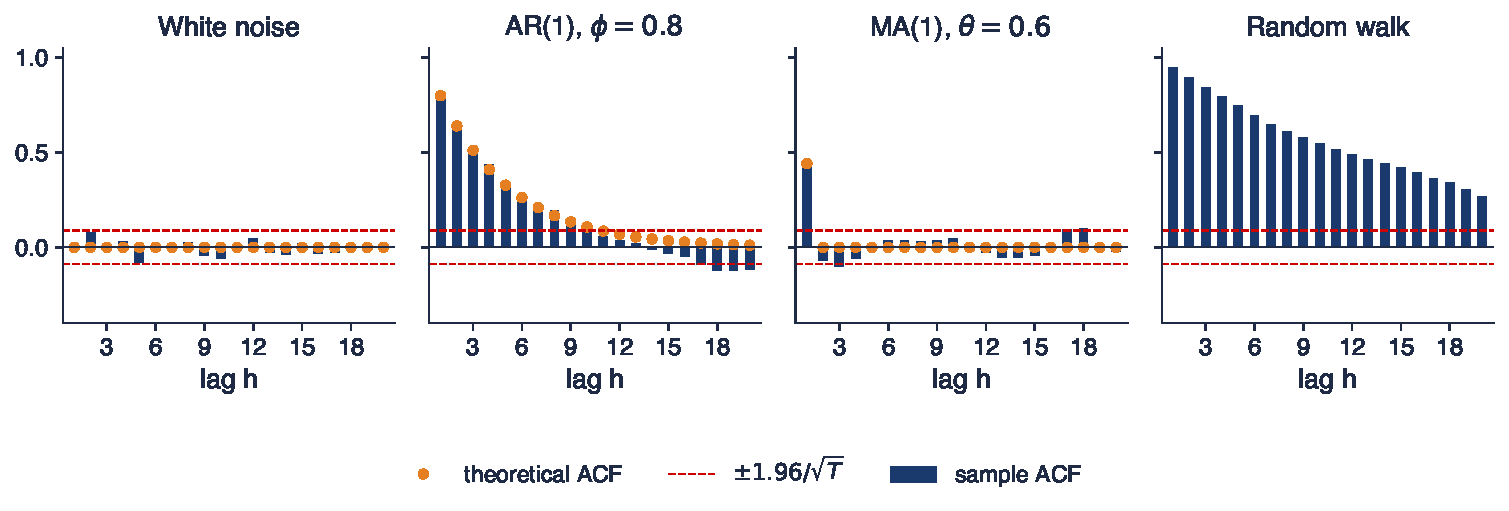
\includegraphics[width=0.97\textwidth,height=0.56\textheight,keepaspectratio]{tsa_ch1_acf_models.pdf}
\end{center}
\vspace{-0.25cm}
\begin{itemize}
    \item $T = 500$ de valori simulate; bare: ACF de selecție; puncte: ACF teoretică; banda $\pm 0{,}088$
\end{itemize}
\quantlet{TSA\_ch1\_acf\_pacf}{\qlurl{TSA_ch1_acf_pacf}}
\end{frame}

\begin{frame}{Interpretarea celor patru corelograme}
\itemsize{\small}
\begin{itemize}
    \item Zgomotul alb: toate barele sînt mici; cea mai mare, $\hat\rho(2) = 0{,}08$, este zgomot
    \item AR(1), $\phi = 0{,}8$: descreștere geometrică, $\hat\rho(1) = 0{,}81$, $\hat\rho(2) = 0{,}65$ (teoretic 0,80 și 0,64)
    \item MA(1), $\theta = 0{,}6$: un singur vîrf, $\hat\rho(1) = 0{,}44$ (teoretic 0{,}44), apoi nimic: ACF \textbf{se anulează} după decalajul 1
    \item Mersul aleator: $\hat\rho(1) = 0{,}95$, încă 0{,}55 la decalajul 10: descreșterea lentă, aproape liniară, a unei serii nestaționare
    \begin{itemize}
        \item ACF de selecție a unui mers aleator nu are corespondent teoretic: $\rho(h)$ nu este definit
    \end{itemize}
\end{itemize}
\end{frame}

\begin{frame}{Autocorelația parțială}
\itemsize{\small}
\begin{itemize}
    \item \textbf{Definiție}: \textbf{PACF} (funcția de autocorelație parțială) la decalajul $h$, $\phi_{hh}$, este ultimul coeficient al celei mai bune prognoze liniare a lui $X_t$ din $X_{t-1}, \dots, X_{t-h}$:
    \begin{itemize}
        \item $X_t = \phi_{h1}X_{t-1} + \dots + \phi_{hh}X_{t-h} + e_t$
        \item corelația dintre $X_t$ și $X_{t-h}$ după eliminarea efectului liniar al decalajelor intermediare
    \end{itemize}
    \item Primele două valori
    \begin{itemize}
        \item $\phi_{11} = \rho(1)$; $\phi_{22} = \dfrac{\rho(2) - \rho(1)^2}{1 - \rho(1)^2}$
        \item cazul general: recursia Durbin--Levinson; PACF de selecție folosește $\hat\rho(h)$ în locul lui $\rho(h)$
    \end{itemize}
    \item \textbf{Exemplu rezolvat}
    \begin{itemize}
        \item AR(1): $\rho(2) = \rho(1)^2$, deci $\phi_{22} = 0$: odată cunoscut $X_{t-1}$, $X_{t-2}$ nu mai aduce nimic
        \item AR(2) cu $\phi_1 = 0{,}5$, $\phi_2 = 0{,}3$: $\rho(1) = 0{,}714$, $\rho(2) = 0{,}657$, $\phi_{22} = (0{,}657 - 0{,}510)/(1 - 0{,}510) = 0{,}300 = \phi_2$
    \end{itemize}
    \item Aceeași bandă ca pentru ACF, în cazul zgomotului alb: $\pm 1{,}96/\sqrt{T}$
\end{itemize}
\end{frame}

\begin{frame}{ACF și PACF pentru trei procese}
\itemsize{\footnotesize}
\begin{center}
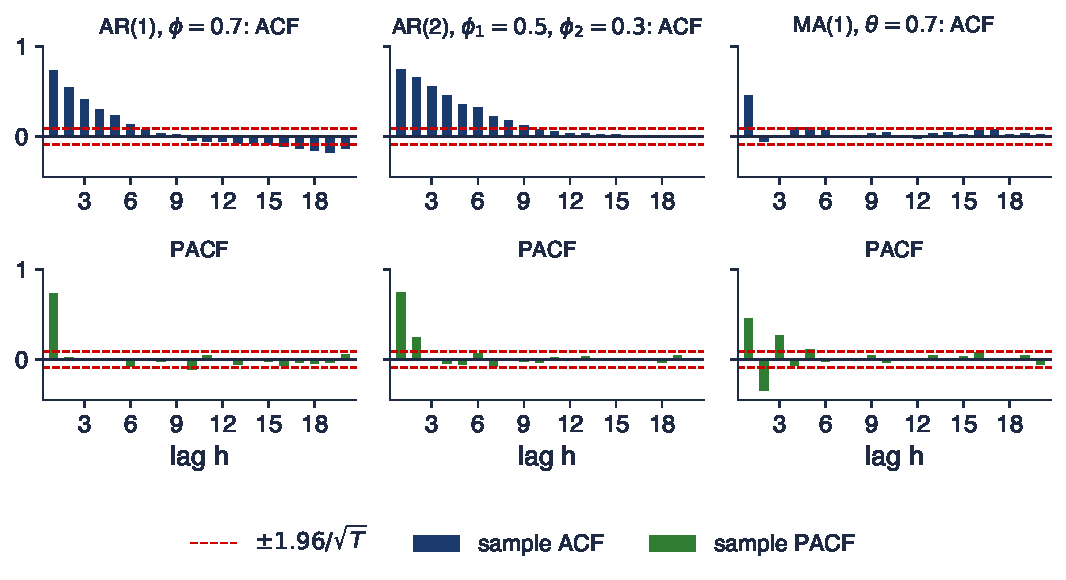
\includegraphics[width=0.97\textwidth,height=0.64\textheight,keepaspectratio]{tsa_ch1_acf_pacf.pdf}
\end{center}
\vspace{-0.25cm}
\begin{itemize}
    \item $T = 500$ de valori simulate din AR(1), AR(2) și MA(1); sus: ACF de selecție; jos: PACF de selecție
\end{itemize}
\quantlet{TSA\_ch1\_acf\_pacf}{\qlurl{TSA_ch1_acf_pacf}}
\end{frame}

\begin{frame}{Interpretarea ACF și PACF}
\itemsize{\small}
\begin{itemize}
    \item AR(1): ACF descrește; PACF are un singur vîrf, $\hat\phi_{11} = 0{,}73$, apoi $\hat\phi_{22} = 0{,}03$
    \begin{itemize}
        \item AR(2): două vîrfuri în PACF, $\hat\phi_{22} = 0{,}24$ (teoretic 0,3), apoi $\hat\phi_{33} = 0{,}01$
    \end{itemize}
    \item MA(1): imaginea în oglindă; un singur vîrf în ACF ($\hat\rho(1) = 0{,}46$), o PACF care alternează și descrește ($-0{,}34$, $0{,}26$, ...)
    \item Regula de identificare din \tsachlink{https://danpele.github.io/Time-Series-Analysis/RO/Cursuri/capitol2_modele_arma.pdf}{Capitolul 2} \refHP:
    \begin{itemize}
        \item PACF se anulează după $p$: AR($p$); ACF se anulează după $q$: MA($q$); ambele descresc: ARMA
    \end{itemize}
\end{itemize}
\end{frame}

\begin{frame}{Date reale: trei piețe}
\itemsize{\small}
\begin{columns}[T]
\begin{column}{0.40\textwidth}
\centering
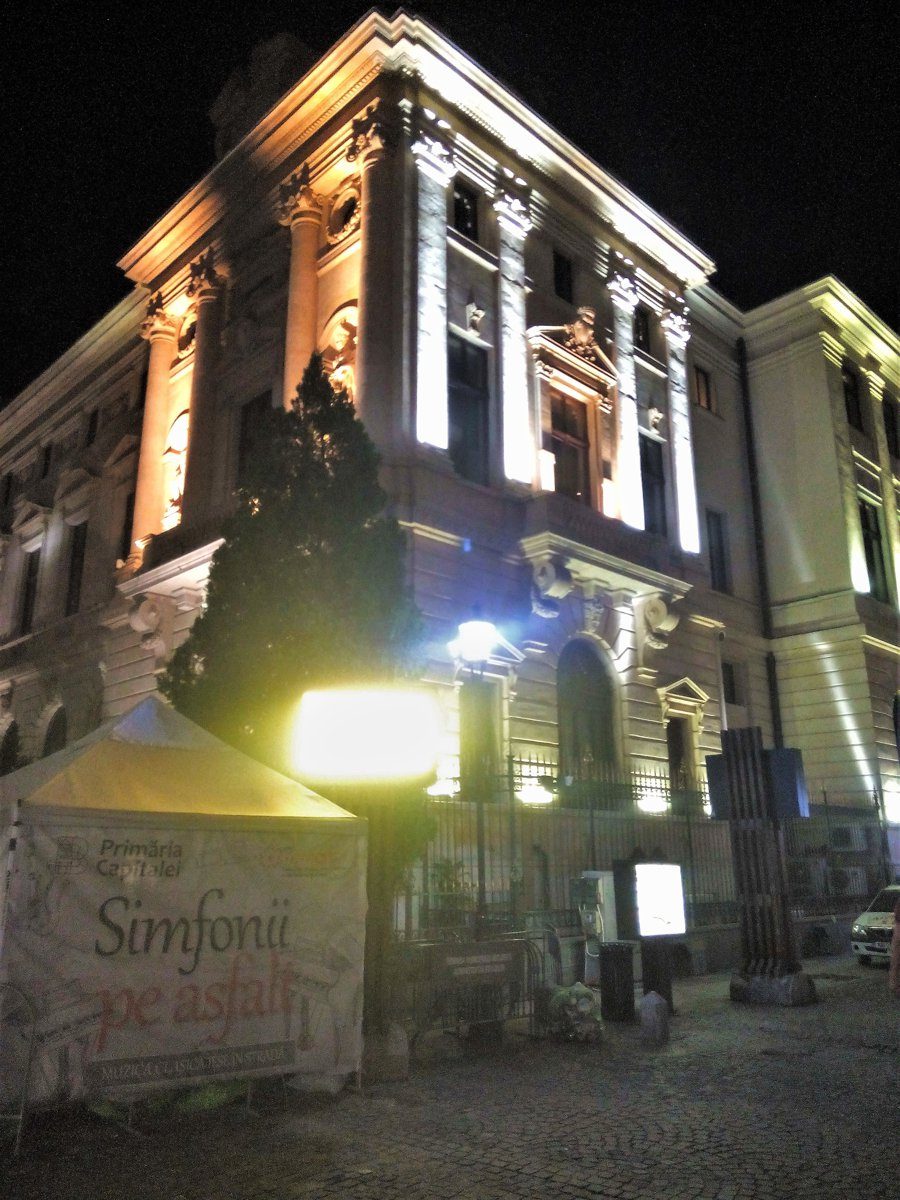
\includegraphics[height=0.48\textheight]{ch1_bnr_2018.jpg}\\[1mm]
\imgcap{Banca Națională a României (BNR), care publică cursul de referință EUR/RON}
\imgcredit{https://commons.wikimedia.org/wiki/File:National_Bank_of_Romania_(old_building),_Bucharest_by_nickispeaki_01.jpg}{Foto: Nickispeaki (2018); CC BY-SA 4.0; Wikimedia Commons}
\end{column}
\begin{column}{0.56\textwidth}
\begin{itemize}
    \item Urmează: ACF a randamentelor logaritmice zilnice ale BET din 2000, a valorilor lor absolute și a pătratelor lor
    \item Aceeași analiză pentru EUR/RON (cursul de referință BNR) și S\&P 500: Seminarul 1, cerința B2
    \item Întrebarea: sînt randamentele BET zgomot alb? De ce tip?
\end{itemize}
\end{column}
\end{columns}
\end{frame}

\begin{frame}{BET: ACF a randamentelor, a valorilor absolute și a pătratelor}
\itemsize{\footnotesize}
\begin{center}
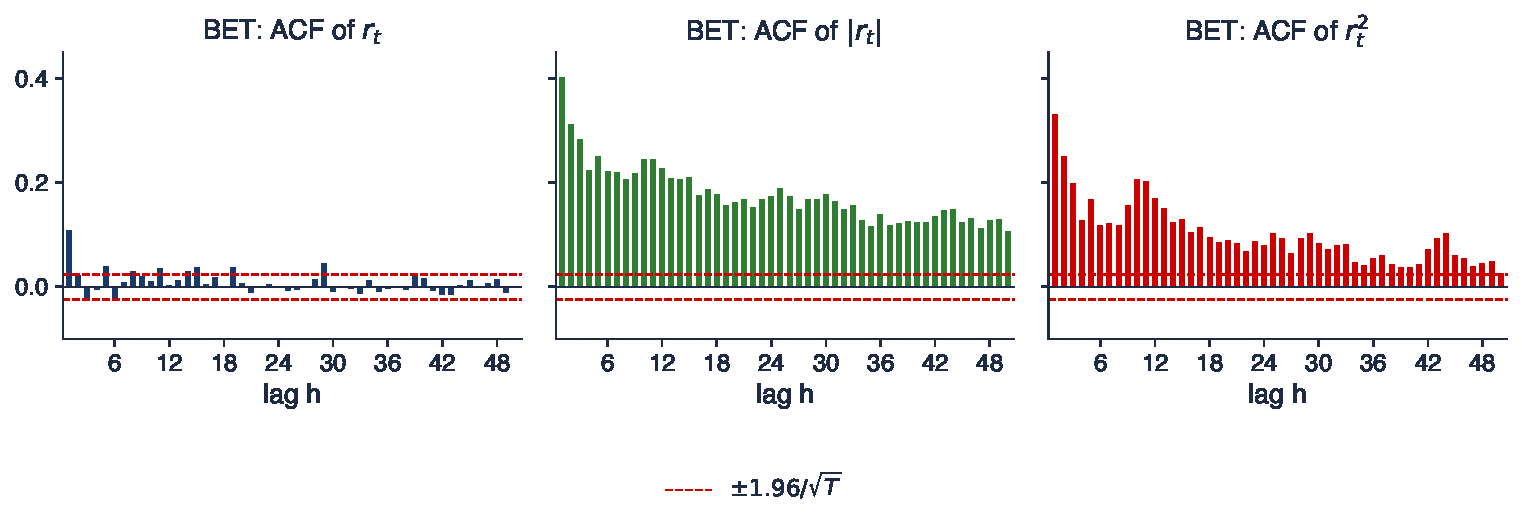
\includegraphics[width=0.97\textwidth,height=0.58\textheight,keepaspectratio]{tsa_ch1_bet_acf.pdf}
\end{center}
\vspace{-0.25cm}
\begin{itemize}
    \item Randamente logaritmice zilnice, 6\,670 de zile, decalajele 1--50; banda $\pm 0{,}024$
\end{itemize}
\quantlet{TSA\_ch1\_acf\_pacf}{\qlurl{TSA_ch1_acf_pacf}}
\end{frame}

\begin{frame}{Interpretarea corelogramelor BET}
\itemsize{\small}
\begin{itemize}
    \item Randamentele: $\hat\rho(1) = 0{,}109$, clar în afara benzii; $Q^*(10) = 108$
    \begin{itemize}
        \item semnificativă statistic, dar mică: randamentul de ieri explică aproximativ $\hat\rho(1)^2 = 1{,}2\%$ din varianța celui de azi
        \item un semn tipic al unei piețe mai puțin lichide (tranzacționare nesincronă)
    \end{itemize}
    \item Valorile absolute: $\hat\rho(1) = 0{,}40$ și încă 0{,}11 la decalajul 50; pătratele: $\hat\rho(1) = 0{,}33$
    \begin{itemize}
        \item mișcările mari urmează după mișcări mari: volatility clustering, o memorie lungă a mărimii randamentelor
    \end{itemize}
    \item Concluzie: randamentele BET sînt apropiate de un zgomot alb \textbf{slab}; media este greu de anticipat, varianța nu (\tsachlink{https://danpele.github.io/Time-Series-Analysis/RO/Cursuri/capitol5_volatilitate_conditionata_garch.pdf}{Capitolul 5})
\end{itemize}
\end{frame}

\begin{frame}{Recapitulare: ACF și PACF de selecție}
\itemsize{\small}
\begin{itemize}
    \item $\hat\rho(h) = \hat\gamma(h)/\hat\gamma(0)$, cu împărțitorul $T$; folosim decalaje pînă la aproximativ $T/4$
    \item Pentru date i.i.d.: $\hat\rho(h) \approx N(0, 1/T)$, banda $\pm 1{,}96/\sqrt{T}$; o bară din 20 iese din întîmplare
    \item PACF: efectul direct al decalajului $h$; AR($p$) se anulează în PACF, MA($q$) în ACF
    \item Randamentele: dependență liniară slabă, dependență neliniară puternică
\end{itemize}
\end{frame}


%=============================================================================
\section{Teste portmanteau: Box--Pierce și Ljung--Box}
%=============================================================================

\begin{frame}{Testarea simultană a mai multor autocorelații}
\itemsize{\small}
\begin{itemize}
    \item $H_0$: $\rho(1) = \dots = \rho(m) = 0$ (seria este zgomot alb pînă la decalajul $m$); $H_1$: cel puțin un $\rho(h) \ne 0$
    \begin{itemize}
        \item un test \textbf{portmanteau}: o singură statistică „poartă” $m$ autocorelații
    \end{itemize}
    \item \textbf{Statistica Box--Pierce}, din \refBP: $Q(m) = T\sum_{h=1}^{m}\hat\rho(h)^2$
    \begin{itemize}
        \item în ipoteza $H_0$, fiecare $\sqrt{T}\hat\rho(h) \approx N(0, 1)$, independente: suma a $m$ pătrate este $\approx \chi^2(m)$
    \end{itemize}
    \item \textbf{Statistica Ljung--Box}, din \refLB: $Q^*(m) = T(T + 2)\sum_{h=1}^{m}\dfrac{\hat\rho(h)^2}{T - h}$
    \begin{itemize}
        \item ponderea $(T + 2)/(T - h)$ corectează varianța mică a lui $\hat\rho(h)$ la decalaje mari; aceeași limită $\chi^2(m)$
    \end{itemize}
    \item Respingem $H_0$ la 5\% dacă $Q^* > \chi^2_{0{,}95}(m)$; de exemplu, $\chi^2_{0{,}95}(10) = 18{,}31$
    \begin{itemize}
        \item pentru reziduurile unui ARMA($p, q$): $\chi^2(m - p - q)$ (\tsachlink{https://danpele.github.io/Time-Series-Analysis/RO/Cursuri/capitol2_modele_arma.pdf}{Capitolul 2})
    \end{itemize}
\end{itemize}
\end{frame}

\begin{frame}{Exemplu rezolvat: statistica Ljung--Box}
\itemsize{\small}
\begin{itemize}
    \item $T = 100$; $\hat\rho(1) = 0{,}25$, $\hat\rho(2) = 0{,}12$, $\hat\rho(3) = -0{,}08$; banda $\pm 0{,}196$
    \begin{itemize}
        \item doar $\hat\rho(1)$ este în afara benzii
    \end{itemize}
    \item Box--Pierce: $Q(3) = 100\,(0{,}0625 + 0{,}0144 + 0{,}0064) = 8{,}33$
    \begin{itemize}
        \item Ljung--Box: $Q^*(3) = 100 \cdot 102\,\big(\frac{0{,}0625}{99} + \frac{0{,}0144}{98} + \frac{0{,}0064}{97}\big) = 8{,}61$
    \end{itemize}
    \item Valoarea critică $\chi^2_{0{,}95}(3) = 7{,}81$: respingem $H_0$; valoarea p este 0{,}035
    \begin{itemize}
        \item seria nu este zgomot alb; dependența este concentrată la decalajul 1
    \end{itemize}
    \item Alegerea lui $m$: prea mic ratează decalajele îndepărtate; prea mare diluează dovezile
    \begin{itemize}
        \item alegeri uzuale: $m = 10$ pentru date nesezoniere, $m = 2s$ pentru date sezoniere cu perioada $s$ \refFPP
    \end{itemize}
\end{itemize}
\end{frame}

\begin{frame}{Box--Pierce și Ljung--Box în eșantioane mici}
\itemsize{\footnotesize}
\begin{center}
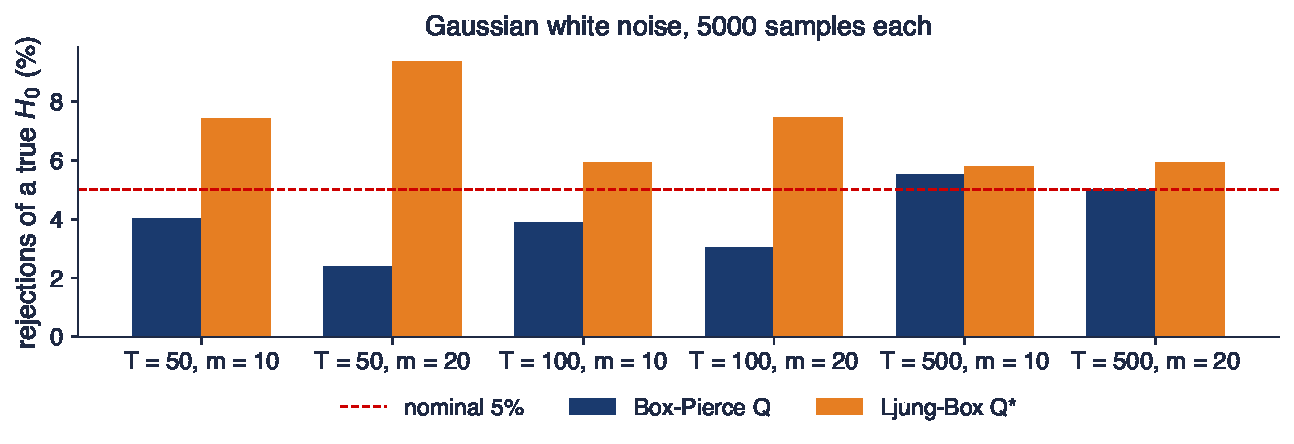
\includegraphics[width=0.97\textwidth,height=0.60\textheight,keepaspectratio]{tsa_ch1_lb_size.pdf}
\end{center}
\vspace{-0.25cm}
\begin{itemize}
    \item Proporția din 5000 de eșantioane de zgomot alb gaussian în care fiecare test respinge o ipoteză $H_0$ adevărată, la nivelul de 5\%
\end{itemize}
\quantlet{TSA\_ch1\_portmanteau}{\qlurl{TSA_ch1_portmanteau}}
\end{frame}

\begin{frame}{Interpretarea simulării mărimii testelor}
\itemsize{\small}
\begin{itemize}
    \item $T = 50$, $m = 20$: Box--Pierce respinge în 2{,}4\% dintre eșantioane, Ljung--Box în 9{,}4\%
    \begin{itemize}
        \item Box--Pierce este prea îngăduitor: ratează dependența; Ljung--Box greșește în sens opus cînd $m$ este mare față de $T$
    \end{itemize}
    \item $T = 500$, $m = 20$: 5{,}0\% și 5{,}9\%: ambele aproape de 5\%
    \item În practică: folosim Ljung--Box (implicit în programe) și păstrăm $m$ mult sub $T$ (de exemplu, $m \le T/5$)
\end{itemize}
\end{frame}

\begin{frame}{Statisticile Ljung--Box pentru serii reale}
\itemsize{\footnotesize}
\begin{center}
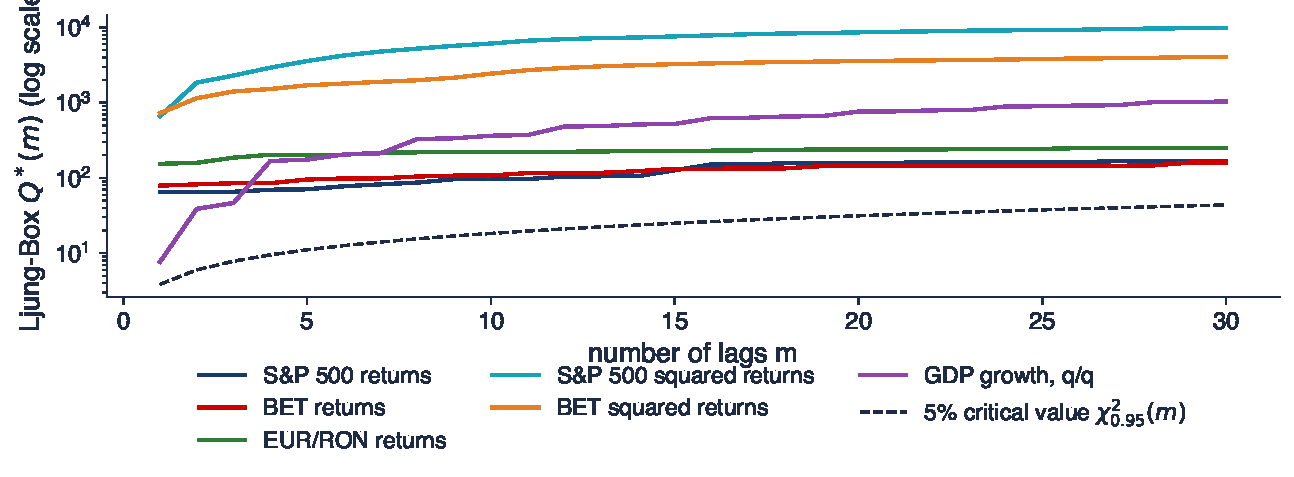
\includegraphics[width=0.97\textwidth,height=0.60\textheight,keepaspectratio]{tsa_ch1_lb_stats.pdf}
\end{center}
\vspace{-0.25cm}
\begin{itemize}
    \item $Q^*(m)$ pentru $m = 1, \dots, 30$ (scară logaritmică), față de valoarea critică de 5\% $\chi^2_{0{,}95}(m)$ (linie întreruptă)
\end{itemize}
\quantlet{TSA\_ch1\_portmanteau}{\qlurl{TSA_ch1_portmanteau}}
\end{frame}

\begin{frame}{Interpretarea statisticilor Ljung--Box}
\itemsize{\footnotesize}
\begin{center}
\scriptsize
\begin{tabular}{lrrrrr}
\toprule
Seria & $T$ & $\hat\rho(1)$ & $\hat\rho(4)$ & $Q^*(10)$ & p \\
\midrule
S\&P 500, randamente zilnice & 6\,714 & $-0{,}10$ & $-0{,}03$ & 96{,}3 & $<$\,0{,}001 \\
S\&P 500, randamente la pătrat & 6\,714 & $0{,}31$ & $0{,}31$ & 6132{,}8 & $<$\,0{,}001 \\
BET, randamente zilnice & 6\,670 & $0{,}11$ & $-0{,}01$ & 108{,}0 & $<$\,0{,}001 \\
BET, randamente la pătrat & 6\,670 & $0{,}33$ & $0{,}13$ & 2440{,}0 & $<$\,0{,}001 \\
EUR/RON, randamente zilnice & 5\,352 & $0{,}17$ & $-0{,}06$ & 221{,}7 & $<$\,0{,}001 \\
PIB România, creștere t/t & 125 & $-0{,}24$ & $0{,}96$ & 364{,}8 & $<$\,0{,}001 \\
PIB România, creștere an/an & 122 & $0{,}63$ & $0{,}03$ & 75{,}0 & $<$\,0{,}001 \\
IAPC România, inflația lunară & 260 & $0{,}40$ & $0{,}12$ & 126{,}7 & $<$\,0{,}001 \\
Nil, debitul anual & 100 & $0{,}50$ & $0{,}24$ & 88{,}1 & $<$\,0{,}001 \\
Pete solare, anual & 309 & $0{,}82$ & $-0{,}28$ & 627{,}4 & $<$\,0{,}001 \\
\bottomrule
\end{tabular}
\end{center}
\begin{itemize}
    \item Toate seriile resping ipoteza de zgomot alb; pentru pătratele randamentelor statistica este de zeci de ori mai mare decît pentru randamente
    \item Respingerea spune doar că există \textbf{o anumită} corelație; ACF arată unde (PIB: decalajul 4, sezonul)
\end{itemize}
\end{frame}

\begin{frame}{Recapitulare: teste portmanteau}
\itemsize{\small}
\begin{itemize}
    \item $Q(m) = T\sum\hat\rho(h)^2$, $Q^*(m) = T(T + 2)\sum\hat\rho(h)^2/(T - h)$; ambele $\approx \chi^2(m)$ pentru zgomot alb
    \item Ljung--Box are o mărime mai bună în eșantioane mici; păstrăm $m$ mult sub $T$
    \item O respingere este un semnal pentru modelare, nu un model; în prezența efectelor GARCH, testul randamentelor respinge prea des
\end{itemize}
\end{frame}


%=============================================================================
\section{Transformări}
%=============================================================================

\begin{frame}{Motivele transformării unei serii}
\itemsize{\small}
\begin{itemize}
    \item Scopuri
    \begin{itemize}
        \item stabilizarea varianței (oscilații sezoniere care cresc odată cu nivelul)
        \item transformarea creșterii exponențiale într-un trend liniar
        \item eliminarea unui trend stochastic sau a unui tipar sezonier (diferențiere)
    \end{itemize}
    \item \textbf{Logaritmul}: $\ln Y_t$; diferența lui este rata de creștere în termeni continui
    \begin{itemize}
        \item $100\,\Delta\ln Y_t \approx$ variația procentuală, pentru variații mici: $\ln 1{,}03 = 0{,}0296$, circa 3\%
        \item nu și pentru cele mari: $\ln 1{,}30 = 0{,}262$, $\ln 0{,}70 = -0{,}357$; variațiile logaritmice se adună în timp, procentele nu
    \end{itemize}
    \item Ordinea operațiilor pentru o serie pozitivă, cu trend și sezonalitate
    \begin{itemize}
        \item întîi logaritmul (varianța), apoi diferențele (trendul, sezonul); niciodată invers
    \end{itemize}
\end{itemize}
\end{frame}

\begin{frame}{PIB-ul real al României: logaritm, creștere trimestrială și anuală}
\itemsize{\footnotesize}
\begin{center}
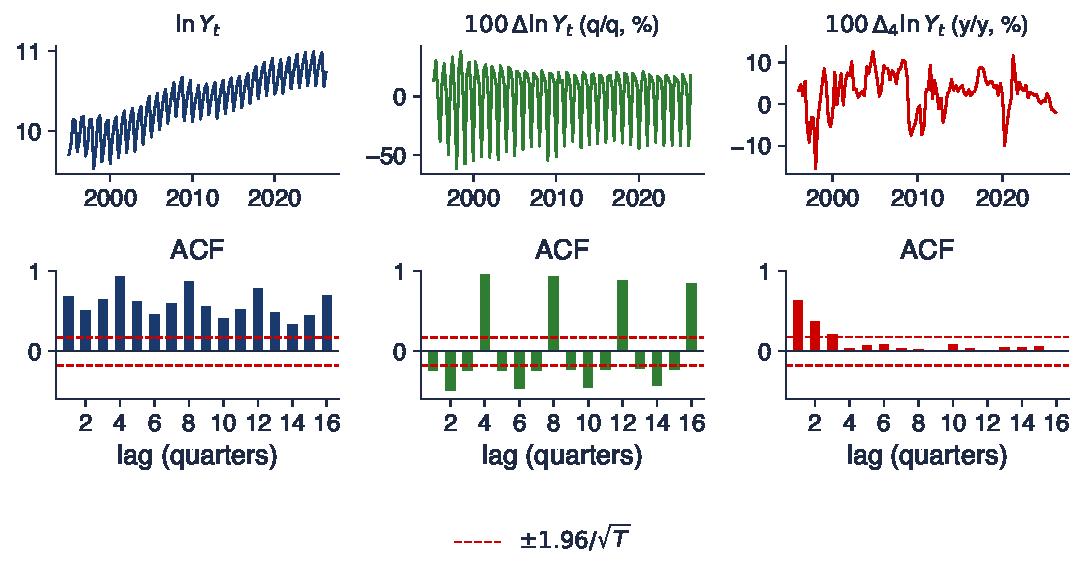
\includegraphics[width=0.97\textwidth,height=0.64\textheight,keepaspectratio]{tsa_ch1_gdp_transform.pdf}
\end{center}
\vspace{-0.25cm}
\begin{itemize}
    \item Date trimestriale, neajustate sezonier, prețuri din 2010 (Eurostat), T1 1995--T2 2026; sus: seriile; jos: ACF de selecție
\end{itemize}
\quantlet{TSA\_ch1\_transformations}{\qlurl{TSA_ch1_transformations}}
\end{frame}

\begin{frame}{Interpretarea transformărilor PIB}
\itemsize{\small}
\begin{itemize}
    \item $\ln Y_t$: ACF 0{,}68 la decalajul 1 și 0{,}87 la decalajul 8, cu vîrfuri la fiecare 4 trimestre: trend și sezon
    \item $\Delta\ln Y_t$: trendul a dispărut, sezonul domină: $\hat\rho(4) = 0{,}96$, $\hat\rho(2) = -0{,}49$; abaterea standard 27{,}5\%
    \begin{itemize}
        \item rata trimestru față de trimestru a datelor neajustate măsoară mai ales sezonul
    \end{itemize}
    \item $\Delta_4\ln Y_t$ (creșterea anuală): media 2{,}7\%, ACF se stinge după 2--3 trimestre ($\hat\rho(1) = 0{,}63$, $\hat\rho(4) = 0{,}03$)
    \begin{itemize}
        \item apropiată de staționaritate, cu persistența ciclului economic; T2 2020: $-9{,}9\%$; ultimul trimestru: $-2{,}0\%$
    \end{itemize}
\end{itemize}
\end{frame}

\begin{frame}{Transformarea Box--Cox}
\itemsize{\small}
\begin{itemize}
    \item \textbf{Definiție} \refBC, pentru $y > 0$: $w = \dfrac{y^\lambda - 1}{\lambda}$ pentru $\lambda \ne 0$, $w = \ln y$ pentru $\lambda = 0$
    \begin{itemize}
        \item $\lambda = 1$: forma nu se schimbă; $\lambda = 0{,}5$: radical; $\lambda = 0$: logaritm; $\lambda = -1$: inversă
        \item continuă în $\lambda$: $(y^\lambda - 1)/\lambda \to \ln y$ cînd $\lambda \to 0$
    \end{itemize}
    \item \textbf{Exemplu rezolvat}: $y = 100$ și $y = 400$
    \begin{itemize}
        \item $\lambda = 0{,}5$: $w = 18$ și $38$; $\lambda = 0$: $w = 4{,}605$ și $5{,}991$
        \item cu cît $\lambda$ este mai mic, cu atît valorile mari sînt comprimate mai mult
    \end{itemize}
    \item Alegerea lui $\lambda$: \refGuerrero, ca în \refFPP
    \begin{itemize}
        \item împărțim seria pe ani; alegem $\lambda$ astfel încît $\mathrm{sd}_i/\mathrm{medie}_i^{1-\lambda}$ să fie cît mai constant de la un an la altul
    \end{itemize}
    \item Prognozele se fac pentru $w$ și se transformă înapoi: $y = (\lambda w + 1)^{1/\lambda}$; valoarea obținută este mediana, nu media
\end{itemize}
\end{frame}

\begin{frame}{Box--Cox pentru PIB-ul nominal al României}
\itemsize{\footnotesize}
\begin{center}
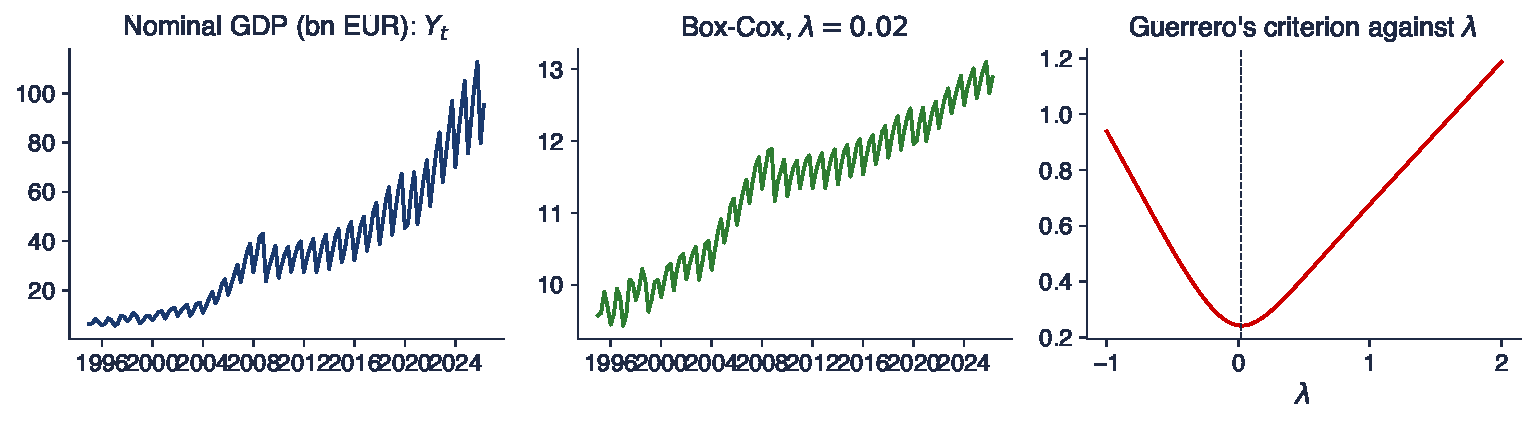
\includegraphics[width=0.97\textwidth,height=0.54\textheight,keepaspectratio]{tsa_ch1_boxcox.pdf}
\end{center}
\vspace{-0.25cm}
\begin{itemize}
    \item PIB-ul nominal trimestrial, neajustat sezonier, de la 6{,}4 la 95{,}2 mld. EUR; criteriul lui Guerrero pe blocuri anuale de 4 trimestre
\end{itemize}
\quantlet{TSA\_ch1\_transformations}{\qlurl{TSA_ch1_transformations}}
\end{frame}

\begin{frame}{Interpretarea alegerii Box--Cox}
\itemsize{\small}
\begin{itemize}
    \item $\hat\lambda$ al lui Guerrero $= 0{,}02$: practic logaritmul (criteriul 0{,}243 la $\hat\lambda$, 0{,}243 la $\lambda = 0$, 0{,}68 la $\lambda = 1$)
    \begin{itemize}
        \item alegem valoarea rotundă și ușor de interpretat: $\lambda = 0$
    \end{itemize}
    \item De ce se potrivește logaritmul: oscilația sezonieră este o proporție stabilă din nivel, circa 39\% în primii cinci ani și 41\% în ultimii cinci
    \begin{itemize}
        \item sezonalitatea multiplicativă devine aditivă după logaritmare
    \end{itemize}
    \item Box--Cox corectează doar varianța; trendul și sezonul tot trebuie eliminate prin diferențiere
\end{itemize}
\end{frame}

\begin{frame}{Supradiferențierea}
\itemsize{\footnotesize}
\begin{center}
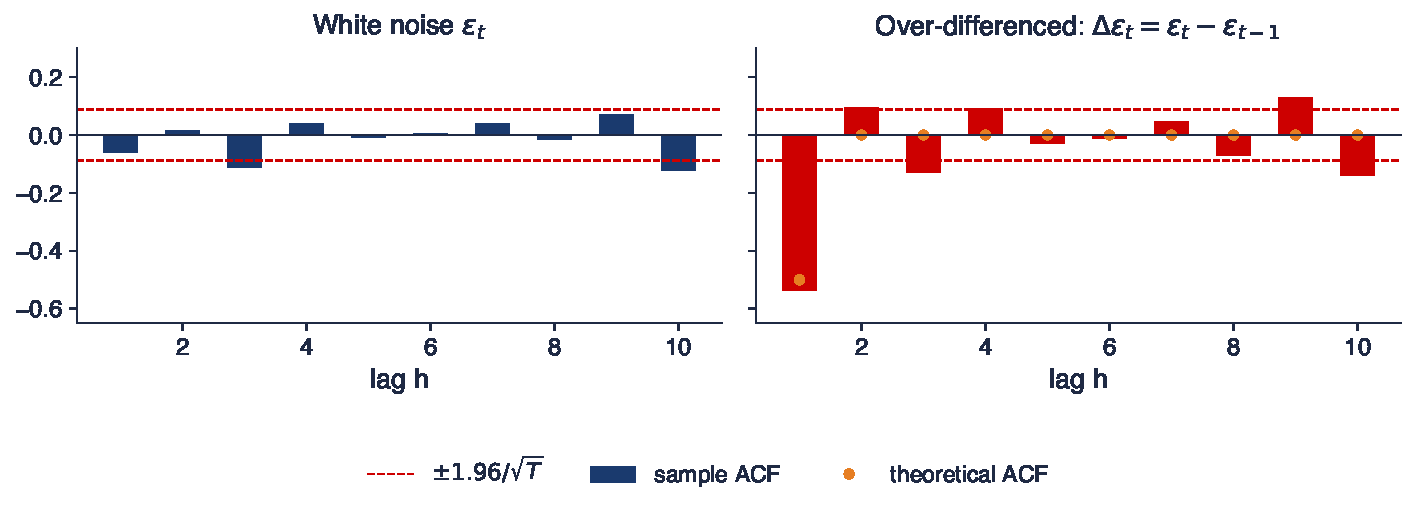
\includegraphics[width=0.97\textwidth,height=0.50\textheight,keepaspectratio]{tsa_ch1_overdiff.pdf}
\end{center}
\vspace{-0.25cm}
\begin{itemize}
    \item ACF de selecție pentru 500 de valori de zgomot alb (stînga) și pentru prima lui diferență (dreapta)
\end{itemize}
\quantlet{TSA\_ch1\_transformations}{\qlurl{TSA_ch1_transformations}}
\end{frame}

\begin{frame}{Interpretarea supradiferențierii}
\itemsize{\small}
\begin{itemize}
    \item $\Delta\varepsilon_t = \varepsilon_t - \varepsilon_{t-1}$ este un MA(1) cu $\theta = -1$: $\rho(1) = -1/2$; aici $\hat\rho(1) = -0{,}54$
    \begin{itemize}
        \item varianța se dublează: 0{,}95 devine 2{,}01
    \end{itemize}
    \item Un $\hat\rho(1)$ puternic negativ, apropiat de $-0{,}5$, după diferențiere: un semn că seria nu avea nevoie de ea
    \begin{itemize}
        \item la fel se întîmplă cu o serie staționară în jurul trendului: $\Delta(a + bt + \varepsilon_t) = b + \varepsilon_t - \varepsilon_{t-1}$
    \end{itemize}
    \item Diferențiem cît este nevoie, nu mai mult; \tsachlink{https://danpele.github.io/Time-Series-Analysis/RO/Cursuri/capitol3_radacini_unitare_modele_arima.pdf}{Capitolul 3} dă testele formale pentru numărul de diferențieri
\end{itemize}
\end{frame}

\begin{frame}{Recapitulare: transformări}
\itemsize{\small}
\begin{itemize}
    \item Întîi logaritmul, pentru seriile pozitive ale căror oscilații cresc cu nivelul; apoi diferențele
    \item $100\,\Delta\ln Y_t$: creșterea în \%; $\Delta_4$, $\Delta_{12}$: creșterea anuală pentru date trimestriale și lunare
    \item Box--Cox cu $\lambda$ ales prin metoda Guerrero; pentru PIB-ul României $\hat\lambda \approx 0$, logaritmul
    \item Supradiferențierea creează $\rho(1) \approx -0{,}5$ și mărește varianța
\end{itemize}
\end{frame}


%=============================================================================
\section{Două serii clasice}
%=============================================================================

\begin{frame}{Studiu de caz: Yule (1927) și Slutzky (1937)}
\itemsize{\small}
\begin{itemize}
    \item \textbf{Întrebarea} anilor 1920: de unde provin ciclurile regulate ale petelor solare și ale activității economice?
    \begin{itemize}
        \item viziunea dominantă: componente periodice ascunse (sume de sinusoide), estimate cu periodograma
    \end{itemize}
    \item \refYule: numărul de pete solare depinde de propriile două valori anterioare plus o perturbație aleatoare
    \begin{itemize}
        \item $X_t = \phi_1X_{t-1} + \phi_2X_{t-2} + \varepsilon_t$: prima autoregresie; un pendul amortizat lovit de șocuri aleatoare
        \item un ciclu fără nicio sinusoidă: șocurile îl întrețin, dinamica îi dă perioada
    \end{itemize}
    \item \refSlutzky: sumele mobile ale unor numere pur aleatoare (o serie de loterie) produc unde netede, asemănătoare ciclurilor
    \begin{itemize}
        \item procesul de medie mobilă (MA) și un avertisment: ciclurile din date pot fi create prin mediere
    \end{itemize}
    \item Moștenirea: procese staționare construite din zgomot alb; \refWold\ a unificat cele două viziuni (secțiunea 4); \refHP, cap.~3
\end{itemize}
\end{frame}

\begin{frame}{Nilul și petele solare}
\itemsize{\small}
\begin{columns}[T]
\begin{column}{0.46\textwidth}
\centering
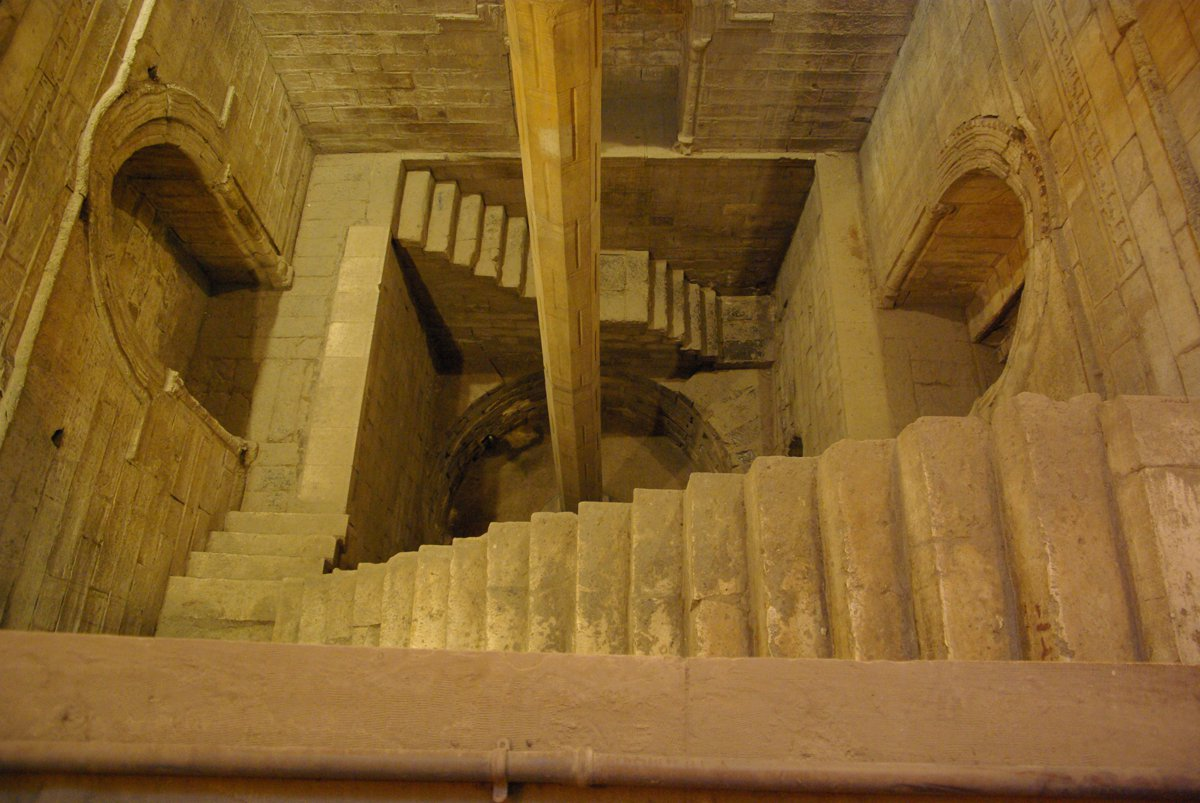
\includegraphics[height=0.44\textheight]{ch1_nilometer_cairo.jpg}\\[1mm]
\imgcap{Nilometrul de pe insula Roda, Cairo: nivelurile Nilului se înregistrează aici de peste o mie de ani}
\imgcredit{https://commons.wikimedia.org/wiki/File:Kairo_Nilometer_BW_1.jpg}{Foto: Berthold Werner (2010); CC BY-SA 3.0; Wikimedia Commons}
\end{column}
\begin{column}{0.50\textwidth}
\begin{itemize}
    \item \textbf{Nilul}: debitul anual la Aswan, 1871--1970, 100 de observații; o scădere în jurul anului 1898 \refCobb
    \item \textbf{Petele solare}: valori anuale, 1700--2008, 309 observații; seria care a inspirat autoregresia \refYule
    \item Ambele sînt incluse în \texttt{statsmodels}; ambele oferă o lecție despre interpretarea ACF
\end{itemize}
\end{column}
\end{columns}
\end{frame}

\begin{frame}{Nilul și petele solare: seriile și ACF}
\itemsize{\footnotesize}
\begin{center}
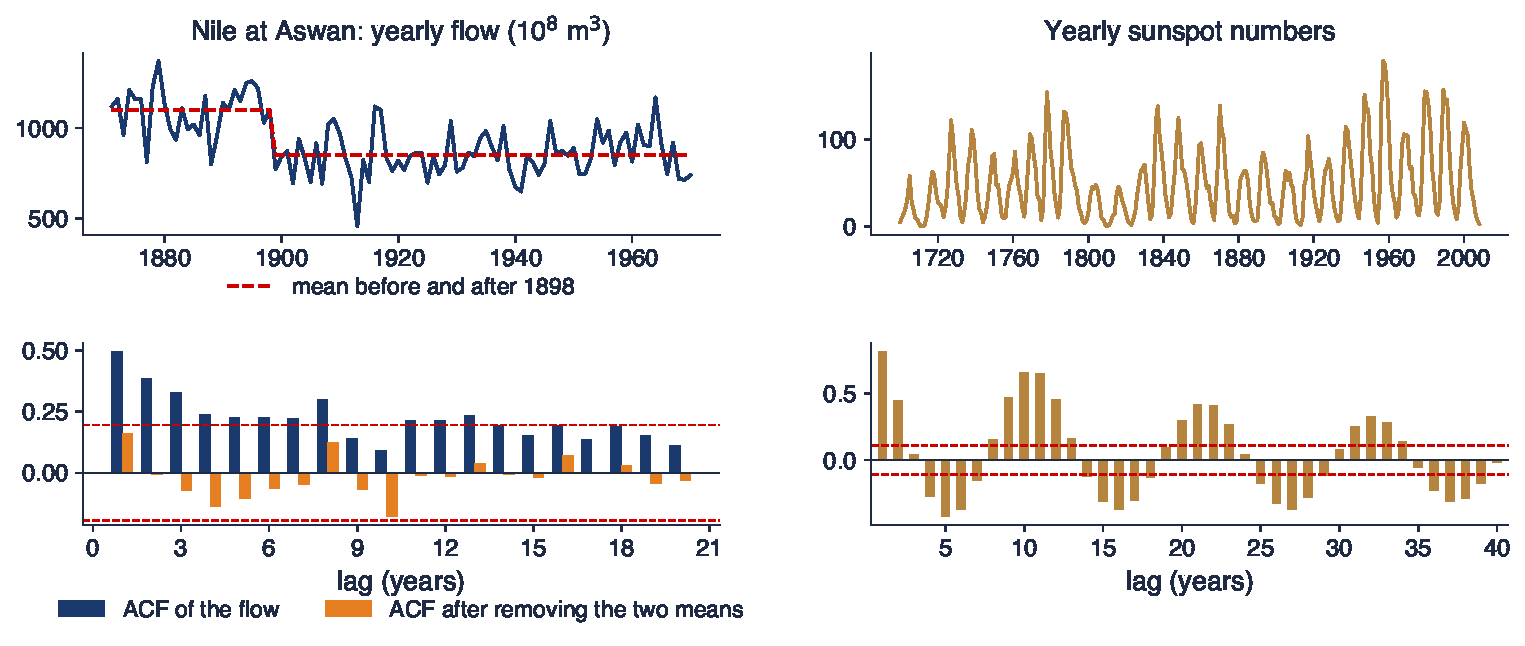
\includegraphics[width=0.97\textwidth,height=0.64\textheight,keepaspectratio]{tsa_ch1_textbook.pdf}
\end{center}
\vspace{-0.25cm}
\begin{itemize}
    \item Stînga: debitul Nilului cu media înainte și după 1898, și două ACF; dreapta: numărul de pete solare și ACF pînă la decalajul 40
\end{itemize}
\quantlet{TSA\_ch1\_textbook\_series}{\qlurl{TSA_ch1_textbook_series}}
\end{frame}

\begin{frame}{Interpretarea celor două serii clasice}
\itemsize{\small}
\begin{itemize}
    \item Nilul: $\hat\rho(1) = 0{,}50$ și o descreștere lentă; $Q^*(10) = 88{,}1$ (p $<$\,0{,}001)
    \begin{itemize}
        \item după eliminarea celor două medii (1098 și 850): $\hat\rho(1) = 0{,}16$, $Q^*(10) = 13{,}0$ (p = 0{,}225)
        \item o ACF care scade lent poate proveni dintr-o \textbf{ruptură}, nu din persistență sau dintr-o rădăcină unitară
    \end{itemize}
    \item Petele solare: o undă amortizată, minim $-0{,}43$ la decalajul 5, vîrf 0{,}66 la decalajul 10
    \begin{itemize}
        \item ciclul solar de circa 11 ani; o serie staționară cu un ciclu, modelată de \refYule\ printr-un AR(2)
    \end{itemize}
    \item Interpretăm ACF împreună cu graficul seriei și cu ce știm despre modul în care au fost produse datele
\end{itemize}
\end{frame}

\begin{frame}{Recapitulare: două serii clasice}
\itemsize{\small}
\begin{itemize}
    \item O ACF care scade lent are mai multe cauze posibile: rădăcina unitară, persistența puternică, ruptura structurală
    \item Ciclurile apar ca unde amortizate în ACF
\end{itemize}
\end{frame}


%=============================================================================
\section{Contribuția posibilă a AI}
%=============================================================================

\begin{frame}{Contribuția posibilă a AI}
\itemsize{\small}
\begin{itemize}
    \item \textbf{Cod}: o primă versiune a unui script care descarcă o serie, o reprezintă grafic împreună cu ACF și PACF și aplică testul Ljung--Box pentru mai multe valori ale lui $m$
    \item \textbf{Explicații}: o a doua explicație a unei definiții sau a motivului pentru care o corelogramă arată într-un anumit fel
    \item \textbf{Explorare}: aceleași diagnostice pe multe serii deodată (toate acțiunile BVB, toate ratele inflației din UE)
    \item Exemplu de prompt
    \begin{itemize}
        \item \aiprompt{Write Python code that loads the Romanian monthly HICP from Eurostat, computes 100 times the monthly log difference since 2005, plots the series with its ACF and PACF up to lag 36, and reports the Ljung-Box statistic for m = 12 and m = 24.}
    \end{itemize}
\end{itemize}
\end{frame}

\begin{frame}{Verificări necesare}
\itemsize{\small}
\begin{itemize}
    \item Împărțitorul lui $\hat\gamma(h)$ ($T$, nu $T - h$) și dacă decalajul 0 este inclus în grafic
    \item Ce benzi sînt desenate: $\pm 1{,}96/\sqrt{T}$ sau benzile Bartlett pentru MA; ele răspund la întrebări diferite
    \item Că testul Ljung--Box se aplică transformării staționare, nu nivelului; și cu $m - p - q$ grade de libertate pentru reziduuri
    \item Că „semnificativ” nu este citit ca „mare” sau „profitabil”
    \item Datele, frecvențele și unitățile seriilor (ajustate sezonier sau nu, baza indicelui, procente sau zecimale)
    \item Fiecare referință citată: trebuie să existe; verificați DOI-ul
\end{itemize}
\end{frame}


%=============================================================================
\section{Rezumat}
%=============================================================================

\begin{frame}{Idei de reținut}
\itemsize{\small}
\begin{itemize}
    \item O serie de timp este o traiectorie a unui proces stochastic; inferența dintr-o singură traiectorie cere staționaritate și ergodicitate
    \item Staționaritatea slabă: media constantă și o autocovarianță care depinde doar de decalaj
    \item Zgomotul alb (slab, i.i.d., gaussian) este piesa de bază; mersul aleator este suma lui cumulată și nu este staționar
    \item ACF și PACF de selecție cu benzile $\pm 1{,}96/\sqrt{T}$; testul Ljung--Box testează simultan mai multe decalaje
    \item Seriile reale au nevoie de transformări: logaritm sau Box--Cox pentru varianță, diferențe pentru trend și sezon
    \item Randamentele: aproape necorelate, dar pătratele lor sînt puternic corelate
\end{itemize}
\end{frame}

\begin{frame}{Formule de reținut}
\itemsize{\small}
{\renewcommand{\arraystretch}{1.4}\begin{center}
\scriptsize
\begin{tabular}{ll}
\toprule
\textbf{Mărimea} & \textbf{Formula} \\
\midrule
Autocovarianța, ACF & $\gamma(h) = \mathrm{Cov}(X_t, X_{t+h})$, \quad $\rho(h) = \gamma(h)/\gamma(0)$ \\
MA(1) & $\gamma(0) = \sigma^2(1 + \theta^2)$, \quad $\rho(1) = \theta/(1 + \theta^2)$, \quad $\rho(h) = 0$, $|h| \ge 2$ \\
AR(1) & $\gamma(0) = \sigma^2/(1 - \phi^2)$, \quad $\rho(h) = \phi^{|h|}$ \\
Mersul aleator & $\mathrm{Var}(X_t) = t\sigma^2$, \quad $\mathrm{Cov}(X_t, X_s) = \min(t, s)\,\sigma^2$ \\
Wold & $X_t = \sum_{j \ge 0}\psi_j\varepsilon_{t-j} + \eta_t$, \quad $\sum_j\psi_j^2 < \infty$ \\
ACF de selecție & $\hat\rho(h) = \sum_{t=1}^{T-h}(x_t - \bar x)(x_{t+h} - \bar x)/\sum_{t=1}^{T}(x_t - \bar x)^2$, \quad $\pm 1{,}96/\sqrt{T}$ \\
PACF & $\phi_{11} = \rho(1)$, \quad $\phi_{22} = (\rho(2) - \rho(1)^2)/(1 - \rho(1)^2)$ \\
Ljung--Box & $Q^*(m) = T(T + 2)\sum_{h=1}^{m}\hat\rho(h)^2/(T - h) \sim \chi^2(m)$ \\
Box--Cox & $w = (y^\lambda - 1)/\lambda$, \quad $w = \ln y$ ($\lambda = 0$) \\
\bottomrule
\end{tabular}
\end{center}
}
\end{frame}

\begin{frame}{Autoevaluare}
\itemsize{\small}
\begin{itemize}
    \item \textbf{Întrebare}: $X_t = \varepsilon_t - 0{,}5\varepsilon_{t-1}$, $\sigma^2 = 4$. Cît sînt $\gamma(0)$ și $\rho(1)$?
    \begin{itemize}
        \item \textbf{Răspuns}: $\gamma(0) = 4 \times 1{,}25 = 5$; $\rho(1) = -0{,}5/1{,}25 = -0{,}4$
    \end{itemize}
    \item \textbf{Întrebare}: o corelogramă cu 40 de decalaje pentru o serie cu $T = 400$ arată două bare ușor în afara lui $\pm 0{,}098$. Este seria corelată?
    \begin{itemize}
        \item \textbf{Răspuns}: nu neapărat: aproximativ 2 din 40 de bare ies din întîmplare; aplicăm testul Ljung--Box
    \end{itemize}
    \item \textbf{Întrebare}: după diferențiere, $\hat\rho(1) = -0{,}48$ și nimic altceva nu este semnificativ. Ce sugerează acest lucru?
    \begin{itemize}
        \item \textbf{Răspuns}: supradiferențiere: seria inițială era probabil deja staționară
    \end{itemize}
    \item Urmează: \tsachlink{https://danpele.github.io/Time-Series-Analysis/RO/Cursuri/capitol2_modele_arma.pdf}{Capitolul 2}, modele ARMA: identificarea cu ACF și PACF, estimarea, diagnosticarea și prognoza
\end{itemize}
\end{frame}


%=============================================================================
\section{Bibliografie}
%=============================================================================

\begin{frame}{Bibliografie}
\itemsize{\tiny}
\begin{itemize}
    \item Bartlett, M. S. (1946). On the theoretical specification and sampling properties of autocorrelated time-series. \textit{Supplement to the Journal of the Royal Statistical Society}, 8(1), 27--41. \href{https://doi.org/10.2307/2983611}{doi:10.2307/2983611}
    \item Box, G. E. P., \& Cox, D. R. (1964). An analysis of transformations. \textit{Journal of the Royal Statistical Society: Series B}, 26(2), 211--243. \href{https://doi.org/10.1111/j.2517-6161.1964.tb00553.x}{doi:10.1111/j.2517-6161.1964.tb00553.x}
    \item Box, G. E. P., \& Pierce, D. A. (1970). Distribution of residual autocorrelations in autoregressive-integrated moving average time series models. \textit{Journal of the American Statistical Association}, 65(332), 1509--1526. \href{https://doi.org/10.1080/01621459.1970.10481180}{doi:10.1080/01621459.1970.10481180}
    \item Brockwell, P. J., \& Davis, R. A. (1991). \textit{Time Series: Theory and Methods} (2nd ed.). Springer. \href{https://doi.org/10.1007/978-1-4419-0320-4}{doi:10.1007/978-1-4419-0320-4}
    \item Brockwell, P. J., \& Davis, R. A. (2016). \textit{Introduction to Time Series and Forecasting} (3rd ed.). Springer. \href{https://doi.org/10.1007/978-3-319-29854-2}{doi:10.1007/978-3-319-29854-2}
    \item Cobb, G. W. (1978). The problem of the Nile: Conditional solution to a changepoint problem. \textit{Biometrika}, 65(2), 243--251. \href{https://doi.org/10.1093/biomet/65.2.243}{doi:10.1093/biomet/65.2.243}
    \item Guerrero, V. M. (1993). Time-series analysis supported by power transformations. \textit{Journal of Forecasting}, 12(1), 37--48. \href{https://doi.org/10.1002/for.3980120104}{doi:10.1002/for.3980120104}
    \item Hamilton, J. D. (1994). \textit{Time Series Analysis}. Princeton University Press. \href{https://doi.org/10.2307/j.ctv14jx6sm}{doi:10.2307/j.ctv14jx6sm}
    \item Huang, C., \& Petukhina, A. (2022). \textit{Applied Time Series Analysis and Forecasting with Python}. Springer. \href{https://doi.org/10.1007/978-3-031-13584-2}{doi:10.1007/978-3-031-13584-2}
    \item Hyndman, R. J., \& Athanasopoulos, G. (2021). \textit{Forecasting: Principles and Practice} (3rd ed.). OTexts. \href{https://otexts.com/fpp3/}{otexts.com/fpp3}
    \item Khintchine, A. (1934). Korrelationstheorie der stationären stochastischen Prozesse. \textit{Mathematische Annalen}, 109, 604--615. \href{https://doi.org/10.1007/BF01449156}{doi:10.1007/BF01449156}
    \item Ljung, G. M., \& Box, G. E. P. (1978). On a measure of lack of fit in time series models. \textit{Biometrika}, 65(2), 297--303. \href{https://doi.org/10.1093/biomet/65.2.297}{doi:10.1093/biomet/65.2.297}
    \item Shumway, R. H., \& Stoffer, D. S. (2017). \textit{Time Series Analysis and Its Applications} (4th ed.). Springer. \href{https://doi.org/10.1007/978-3-319-52452-8}{doi:10.1007/978-3-319-52452-8}
    \item Slutzky, E. (1937). The summation of random causes as the source of cyclic processes. \textit{Econometrica}, 5(2), 105--146. \href{https://doi.org/10.2307/1907241}{doi:10.2307/1907241}
    \item Wold, H. (1938). \textit{A Study in the Analysis of Stationary Time Series}. Almqvist \& Wiksell. \href{https://archive.org/details/in.ernet.dli.2015.262214}{archive.org}
    \item Yule, G. U. (1927). On a method of investigating periodicities in disturbed series, with special reference to Wolfer's sunspot numbers. \textit{Philosophical Transactions of the Royal Society A}, 226, 267--298. \href{https://doi.org/10.1098/rsta.1927.0007}{doi:10.1098/rsta.1927.0007}
\end{itemize}
\end{frame}

\end{document}
